\documentclass[technologies,article,submit,pdftex,moreauthors]{Definitions/mdpi}

\firstpage{1}
\makeatletter
\setcounter{page}{\@firstpage}
\makeatother
\pubvolume{1}
\issuenum{1}
\articlenumber{0}
\pubyear{2026}
\copyrightyear{2026}
\datereceived{}
\daterevised{}
\dateaccepted{}
\datepublished{}

\usepackage{adjustbox}
\usepackage{tikz}
\usepackage{placeins}
\usetikzlibrary{arrows.meta,positioning}

\Title{Experimental Characterization of a Low-Cost IoT Electrical Monitoring System for Traceable Machine-Level Energy Performance Indicators}

\Author{Andrés Viveros $^{1}$, Ivan Derpich $^{1,}$*, Juan Miguel Sepúlveda $^{1}$ and Armando Meza $^{1}$}
\AuthorNames{Andrés Viveros, Ivan Derpich, Juan Miguel Sepúlveda and Armando Meza}

\address{$^{1}$ \quad Centre for Innovation in Technology and Design of Materials for the Built Environment (CIMAC), ANID CTI250005, and Department of Industrial Engineering, Faculty of Engineering, Universidad de Santiago de Chile, Santiago, Chile}
\corres{Correspondence: ivan.derpich@usach.cl}

\abstract{
Low-cost IoT-based electrical monitoring technologies enable machine-level energy management, particularly in industrial environments where conventional instrumentation may be economically prohibitive. However, their practical adoption requires experimentally characterized measurement performance and traceable 
integration of electrical data into energy performance indicators (EnPIs). This study presents the experimental characterization of EnPi, a low-cost single-phase electrical monitoring system integrating a commercial PZEM-004T sensing module, an ESP32S3 communication unit, and a provenance-aware data workflow for machine-level EnPI 
calculation. We evaluated ten controlled load conditions and obtained 10,596 records with matching timestamps. We used the Metrel MI2883 power-quality analyzer as the reference instrument. 9,119 pairs of measurements were available for nonzero-load conditions. The system's mean absolute error was 11.41 W, the mean bias was -11.03 W, the mean absolute percentage error was 3.86\%, and the Pearson correlation was 0.9998. The relative errors were highest at low power. For matched time periods with non-zero energy usage, the accumulated energy differences ranged from -8.397\% to -0.235\%. These differences were partly due to the sensing module's 1 Wh energy register resolution. We also conducted a 17-day study in a food-sector environment to show how to derive machine-level energy performance indicators from monitored energy consumption and a company-provided constant production volume of 44 kg per day. The median daily energy performance indicator (EnPI) was 0.0222 kWh/kg, and the production-weighted value was approximately 0.0240 kWh/kg. Together, the work presents a defined experimental assessment of measurement performance and a repeatable, traceable process linking electrical sensing, data collection, and energy reporting. The results indicate that operational monitoring is feasible under the single-phase conditions tested. They do not establish suitability for wider industrial use or metrological certification.}
\keyword{industrial sensors; electrical sensing; IoT metering; active-power measurement; energy performance indicator; machine-level monitoring; data provenance; low-cost sensing}
\featuredapplication{The characterized sensing node supports bounded machine-level electrical monitoring by linking low-cost measurements with production records, provenance metadata, and traceable energy performance indicators.}

\setlength{\headheight}{20pt}

\begin{document}
\section{Introduction}
\label{sec:introduction}

Electrical sensing at the machine level could also enable consideration of energy use at the operating decision scale. But instrumentation for small and medium industrial enterprises is challenged by cost, installation complexity, fragmented production records, and the need for equipment-level data governance, all of which limit monitoring. Consequently, energy data typically appears as aggregates on electricity bills, in manual records, or, at best, as periodic spot measurements, rather than traceable evidence by individual machines, production runs, and process indicators. Cheap IoT metering offers a tempting toe in the door, but throwing cheap sensing nodes at industrial energy monitoring isn’t as simple as plugging a commercial module into a dashboard. First, the sensing node needs to be experimentally characterized against a reference instrument to establish error, bias, detection limits, and continuity constraints under the pre-specified operating conditions. Second, the measurements produced must be traceable from the raw payload to the green indicator, at which point they become an EnPI-calculated number without auditable provenance. The pertinent gap then is not simply a lack of meters or dashboards in and of themselves; rather, it is more fundamentally about the instrumentality of the formation of refined low-cost sensor-to-indicator chains (within which characterized equipment-level measurements are able to be "bridged" to production records and provenance metadata, that is the source of the sustainable competitive advantage), (the process of industrialization and commercialization of the prototype). IoT-based EMS are reported to collect the electric energy consumption data, send the data to digital platforms, and support monitoring \cite{ref1}, \cite{ref4}. Industrial Energy Management System (IEMS) paradigms also emphasize integrating data collection, analysis, indicators, and decision-making \cite{ref2}, \cite{ref3}. 

Nevertheless, many such contributions either focus on digital energy-management architectures without detailed low-cost node characterization or validate acquisition hardware without connecting the measurement layer to production denominators and traceable EnPI calculation. From a technology-development perspective, the key question is how to experimentally characterize a low-cost single-phase electrical monitoring system and integrate it into a reproducible data workflow that preserves measurement provenance through machine-level energy performance indicator calculation. Recent studies provide more specific benchmarks for low-cost electrical metering: wireless power-quality meters, open-source smart meters, calibrated prototypes, device-level IoT meters, and multi-port monitoring systems have been designed and evaluated in different application settings \cite{r3_sousa2023,r3_openz2018,r3_calibration2019,r3_iotmeter2022,r3_conti2023}. Their differing measurement architectures and validation protocols make direct numerical accuracy comparisons inappropriate without matching loads, reference channels, and time windows. The present work instead reports its own bounded agreement study and links those readings to a production-normalized indicator.

This study addresses two evaluation questions. \textbf{RQ1}: What level of agreement does a low-cost single-phase IoT electrical sensing node achieve against a reference analyzer for voltage, current, frequency, power factor, and active power under the tested conditions? \textbf{RQ2}: Can the resulting measurements be linked with production records through a provenance-aware workflow to calculate a machine-level EnPI in a bounded industrial application?

The paper's scope should be read narrowly. EnPI is described as an electrical sensing platform with component-level evaluation against a reference instrument, along with a deployed data-provenance workflow. Platform-level claims pertain to the data model, the logic for source identification, the user-facing modules, and the integration of production and IoT records. Experimental claims relate only to the evaluated single-phase sensing element, the direct-power and interval-energy comparisons, and the 17-day field run.
This comparison should not be taken as a full factory test; it is constrained to single-phase loads, it does not represent systems with variable frequency drives or large loads, and it does not permit the device to be treated as a metrological instrument.
The novelty of the work is not in a sensing principle, a new PZEM-based device, or the first application of production-normalized energy indicators.Previous work has investigated PZEM-based monitoring and EPUs metrics; however, their instruments, methods, and context vary, and consequently their errors are not presented in a way that establishes application dominance across studies. Instead, this study provides a bounded experimental characterization of one low-cost single-phase node and a separate, provenance-aware demonstration of reconstructing measurements into indicators. In particular, this article makes the following contributions:
\begin{enumerate}
\item an integrated single-phase sensing node that acquires electrical variables and transmits time-stamped, source-identified observations to a remote data service;
\item a component-level analysis versus a Metrel MI2883 benchmark device on ten loads with 10,596 temporally paired samples of agreement, error, and completeness of data analyses;
\item an empirical study of active power with 9,119 paired nonzero-load samples for the Metrel \texttt{P1+(Med)} channel, as well as a scenario-based evaluation of accumulated energy which addresses no-load/low-load case scenarios explicitly;
\item a provenance model that relates each observation to the meter, machine, acquisition source, production record, analysis period, and EnPI resulting from it; and
\item a 17-day bounded operational demonstration showing the traceable connection between machine-level measurements, declared daily production, kWh/kg indicators, operational reference values, and rule-based status flags.
\end{enumerate}

\section{Related Work}
\label{sec:related-work}

The related literature for this study centers on a sensor-system question, pursued here descriptively: how inexpensive electrical measurements are obtained, verified, communicated, used to inform decisions, and converted into demonstrable indicators. Accordingly, we consider five lines of inquiry: IoT-based energy management systems, data-driven industrial energy management, web-based platforms and interoperability, equipment-level distributed metering, and regulatory energy performance indicator-based traceability. From this perspective, this organization distinguishes works based on electrical acquisition from those that integrate sensing, production denominators, data provenance, and limited operational use. 

\subsection{IoT Systems for Energy Management}
\label{subsec:iot-systems-energy-management}

Saleem et al. \cite{ref1} present the design and implementation of an IoT-based Smart Energy Management System, where smart meters, middleware, and a user application enable electricity consumption monitoring and support conservation decisions. Saleem et al. \cite{ref4} later extend this perspective to an IoT-integrated energy management system with cyber-physical systems, cloud middleware, and query APIs, measuring variables such as voltage, current, energy, power, and power factor. 
While these results are promising for distributed acquisition and digital representation, they address energy monitoring and operational response, not the quantitative characterization of a low-cost node in a repeatable sensor-to-indicator chain. As a hardware baseline, Varela-Aldás et al. also performed multi-day comparisons of a two-channel PZEM-004T V3.0 AC monitoring solution against a commercial IoT energy monitor for 7 days \cite{ref24}. Their power and energy comparisons show cost feasibility of electrical acquisition, but they neither characterize the EnPi node nor validate the product-normalized, provenance-aware EnPi process. EnPi is unique in that it considers the low-cost node and the data flow as one sensing system. The node is calibrated against a reference analyzer, and the workflow maintains the provenance for every reading until the machine-level EnPi calculation. Therefore, the deliverable is a bounded, repeatable sensor-to-indicator chain, not a standalone electrical sensor or a generic dashboard. Some recent industrially relevant deployments exist, albeit with different techniques. Khasawneh et al. studied a pharmaceutical manufacturing IoT submetering solution that included industrial meters, a gateway, and cloud analytics \cite{r2_khasawneh2025}. Mirani et al. demonstrated industrial energy metering with edge processing and measurement of consumption metrics through wired and wireless meters \cite{r2_mirani2024}. These results are promising for practical application of energy data at the equipment level, but neither shows measurement accuracy for the EnPi single-phase node. Nevertheless, the authors assert concordance between the reference and test instruments in some cases and separately present the source of the production-normalized indicators.  

\subsection{Industrial Energy Management, Data, and Indicators}
\label{subsec:industrial-energy-management}

Ullah et al. \cite{ref2} have presented a high-level descriptive model of IEMS for a smart factory application based on IoT, big data, and analytics. Their approach enables end-to-end energy monitoring, from collecting data at the machine level to delivering insights to energy managers. Li et al. \cite{ref3} present a practical evaluation of an IoT-based industrial EMS employing AHP and fuzzy logic, suggesting that industrial energy management should consider operational indicators and equipment assessment. This matters because energy management can now evolve from standalone measurement to analysis, prioritization, and decision-making. However, these approaches tend to assume certain levels of instrumentation, integration, and digital maturity that are not always available in small and medium-sized industrial enterprises. The EnPi gap is pragmatic: it lets a company move from invoicing, paper-based records, and one-off measurements to managing with auditable data, without instrumenting the entire plant on day one. This phased adoption is essential to address cost limitations, complexity, and dependence on experts. 

\subsection{Web Platforms, Interoperability, and Industrial Digitalization}
\label{subsec:web-platforms}
Kim et al. \cite{ref5} introduce a web-based IoT network architecture with services, RESTful APIs, real-time monitoring, and secure orchestration. Their end users are industrial batteries, but the paper highlights the challenge of building scalable web layers that support heterogeneous devices, integrate data, and deliver digital services. Other pertinent works in smart energy grids, digital twins, cyber-physical systems, and demand response \cite{ref6}, \cite{ref10}, \cite{ref11} demonstrate an emerging pattern in energy systems towards digitized systems and advanced models for operation and decision-making. IoT literature reviews also show the variety of embedded applications, connectivity solutions, and implementation challenges that drive modular monitoring architectures \cite{ref12,ref13}. From an industrial information integration perspective, these architectures require heterogeneous hardware, software, data, organizational, and operational components to exchange information through explicit interfaces and traceability rules. IoT architecture papers for energy-related smart buildings and electric power systems highlight the need for sensing, networking, cybersecurity, services, energy management 
applications, and avoiding measurement being treated as a separate layer \cite{ref27,ref28}. But many advanced digital architectures are designed for environments with lots of data, reliable connectivity, mature industrial integration, and skilled people. EnPi is more incremental; it aims to provide the absolute minimum traceability required to connect every measurement to the company, building, meter, piece of equipment, data source, time, and production. This design choice enables the platform to create a bridge between simple energy records and more advanced management or automation systems. 

\subsection{Distributed Equipment-Level Metering and Machine-Level Monitoring}
\label{subsec:machine-level-monitoring}
Energy consumption can be directly metered or can be estimated at the equipment level via non-intrusive load monitoring (NILM). Classic NILM methods, for example Hart's \cite{ref21}, estimate the power demand of individual appliances from total household demand. This can help when it is not feasible to place meters on each piece of equipment, but it adds uncertainty to load inference and depends on event detection or electrical-signature models. EnPi uses a novel architecture: single-phase sensing nodes positioned at machines, work cells, or at the load points. This means less disaggregation of aggregate readings, and it's possible to trace each reading to the physical measurement point. The tradeoff is that sensors must be installed at these locations, so installation should be incremental. Initial focus can be on equipment with significant energy consumption, production significance, or uncertain consumption. Rather than developing NILM as an indirect inference technique, this paper treats partial metering as a practical means of making energy management decisions based on improved information. 
\subsection{EnPI Indicators, Energy Management Standards, and Traceability}
\label{subsec:enpi-standards}
Energy management is much more than just kWh metering. ISO 50001:2018 describes energy management system requirements and supports continuous improvement in energy performance through processes, objectives, monitoring, and review \cite{ref19}. Further, though related to and aligned with ISO 50001 and ISO 50003, ISO 50006 is complementary and consistent, and it provides detailed guidance on developing the EnB and the EnPI \cite{ref20}. Thus, these arrangements facilitate associating electric metering with operational variables, production, analysis periods, and objective references.
As such, EnPI is regarded as a service architecture for developing and monitoring EnPI indicators. The platform does not claim to validate conformity with the standard; instead, it provides a line of evidence to support operational control, internal reporting, and energy information preparation. Traceability of data origin, date, device, capture method, associated equipment, and production unit makes IoT and manual records reliable inputs for energy-performance analysis.

\subsection{Security, Privacy, and Sustainability of IoT Nodes}
\label{subsec:security-privacy}
IoT integration in energy systems introduces challenges related to security, privacy, and service availability. Abir et al. \cite{ref6} present IoT weaknesses in smart energy systems, and Santo et al. \cite{ref7} address the privacy of shared energy information. Moreover, the works on Green IoT and energy harvesting \cite{ref8}, \cite{ref9} say that field nodes should consider their own consumption, maintenance, and continuity. EnPi generalizes these into evolution requirements, particularly when the number of deployed nodes, or the criticality of instrumented points, grows.
The platform in its present form offers minimal operational security: user login, logical separation of data by company, each meter linked to a company instance, and communication to the server via HTTPS. For the duration of the comparative campaign, we chose an ESP32S3 as the node firmware's transmission unit, read the PZEM module via serial, and forwarded each reading directly to the ingestion endpoint, without an intermediate backend transformation layer for storage. After temporal acquisition discontinuities were detected in the course of the campaign, an alternate firmware branch included the following features: assisted provisioning, remote configuration, locally caching non-transmitted readings in RAM and using a LittleFS-based circular flash queue for storing non-transmitted data, retransmission in chronological order upon recovery of connectivity, and capability for OTA firmware updates. This operational-continuity enhancement was not used to retrospectively modify the validation samples. The logic for buffering and resending is shown in Supplementary Algorithm S1 and Supplementary Fig. S7. The prototype's OTA maintainability feature is not a validated industrial cybersecurity architecture, since the examined branch uses HTTPS transport without certificate pinning. Future versions should improve device-server authentication, credential rotation, secure provisioning, certificate validation, signed firmware, security event logging, and long-term update practices. 
\subsection{Gap Synthesis}
\label{subsec:gap-synthesis}
Previous research has contributed significantly to smart metering, energy IoT, web platforms, industrial digitalization, privacy, sensing-node sustainability, and energy performance indicators. These studies each offer a piece of the puzzle, such as measuring electricity, node performance, data transfer, production environment, data provenance, and EnPI computation. The gap addressed in this paper is more nuanced than a blanket statement that prior systems lack these abilities: the performance of this EnPI node with respect to the named reference channels has been scarcely evaluated experimentally, and a separate procedure that ties stored measurements with enterprise-reported production to compute EnPI values is inadequately documented. This is a difference in availability of evidence, not a statement that this has never been done before or that EnPI is the first platform that integrates metering with production. It considers two particular questions: to what extent this EnPI sensing node measures up to the given reference channels in the presence of invalid data pairs and time intervals, and whether its recorded measurements in a different way-bounded case can be mapped to a production-normalized indicator. To address these questions, we present two related demonstrations rather than a complete end-to-end proof. The enterprise provided a production quantity of 44 kg/day for the industrial case, which was not independently verified. Therefore, the case does not validate a production model or demonstrate that an energy-saving measure saved energy costs; rather, it demonstrates traceability and descriptive EnPI. Details of the relevant literature review and its connection to the EnPI gap are presented in Supplementary Table S1. Table~\ref {tab: positioning} summarizes the two most related classes of previous work to illustrate the bounded integration considered here. The table evaluates the primary contribution represented by each exemplar and should not be interpreted as evidence that every study within a class lacks other capabilities.
\begin{table}[!h]
\caption{Evidence-based positioning relative to selected related work; blank or limited scope must not be interpreted as proof that an individual study lacks a capability.}
\label{tab:positioning}
\centering
\small
\begin{tabularx}{\textwidth}{p{0.17\textwidth}X X X}
\toprule
Study & Primary evaluated contribution & Connection between energy and production & Traceability or sensing-system emphasis \\
\midrule
Saleem et al. \cite{ref1,ref4} & IoT energy acquisition, middleware, and monitoring & Not the central evaluated contribution & Smart-energy monitoring and system integration \\
Ullah et al. \cite{ref2} & Conceptual industrial energy-management framework & Included conceptually in the management process & Data and analytics framework \\
Li et al. \cite{ref3} & IoT-based energy-management evaluation & Energy-management indicators and assessment & Decision-oriented system evaluation \\
Kim et al. \cite{ref5} & Web framework for industrial IoT services & Application-specific rather than EnPI-oriented & Web integration and service orchestration \\
Varela-Aldas et al. \cite{ref24} & Low-cost monitoring of AC electrical variables & Not the primary contribution & Electrical acquisition and device validation \\
Khasawneh et al. \cite{r2_khasawneh2025} & Industrial IIoT submetering and cloud analytics & Operational industrial energy context & Industrial architecture and analytics; no cross-device accuracy inference \\
Mirani et al. \cite{r2_mirani2024} & Industrial edge processing and consumption metrics & Derived consumption metrics & Industrial monitoring integration; not an EnPi-node validation \\
Beisheim et al. \cite{r3_hierarchy2020} & Hierarchical energy performance indicators & Explicit energy-performance indicator hierarchy & Indicator construction rather than low-cost electrical node validation \\
This study & Low-cost node characterization plus measurement-to-EnPI workflow & Daily energy linked with enterprise-declared production in a 17-day traceability case & Reference-instrument comparison, provenance model, and bounded operational demonstration \\
\bottomrule
\end{tabularx}
\end{table}

\subsection{Recent Metering and Industrial EnPI Evidence}
\label{subsec:recent-metering-enpi}

Recent low-cost energy-monitoring platforms integrate metering, heterogeneous device interfaces, dashboards, and cloud connectivity \cite{r3_khan2024}; industrial edge/cloud studies include acquisition and anomaly-monitoring functions \cite{r3_iiot2022}. These implementations offer a useful design benchmark, but their published hardware performance and network results are not directly applicable to the current EnPi node without verification. The most relevant comparison is still the PZEM-based study mentioned previously \cite{ref24}, and the present work further details the choice of reference channel, excluded data, and the provenance of sensors to indicators. At the indicator layer, hierarchical EnPI aggregation in continuous production and industry-specific models for kraft-pulp and engineering manufacturing show the importance of production context, operational boundaries, and relevant variables \cite{r3_hierarchy2020,r3_kraft2021,r3_rubber2020}. Empirical work on Korean industrial EnPI selection and rubber manufacturing further shows that the energy-to-output ratio is one of several possible indicators rather than a universally sufficient causal model \cite{r3_korea2021,r3_piccioni2024}. SME-oriented energy-efficiency assessment frameworks and reviews of manufacturing expert systems offer broader decision-support perspectives \cite{r3_atenea2025,r3_review2024}. A recent multistage test for industrial EnPI selection highlights the risk of treating an unadjusted energy/production ratio as a fully validated baseline \cite{r3_enpi2026}. Accordingly, this study presents the single-machine kWh/kg series as a descriptive, bounded operational indicator, not a production-adjusted causal savings estimate or a statistically validated predictive baseline.

\section{Study Positioning and Evaluation Scope}
\label{sec:research-gap}

The review highlights relevant contributions in IoT metering, smart meters, industrial energy management systems, equipment assessment, privacy, node sustainability, and advanced energy-system technologies. However, these works tend to address these dimensions separately, even though, in practice, they must operate in an integrated way: manual and billing records, granular IoT metering, production records, data-origin traceability, EnPI calculation, progressive adoption according to company digital maturity, and support for operational decision-making.

The practical problem is therefore not the absence of commercial meters or dashboards. The problem addressed here is implementing a reproducible chain that keeps a measurement linked to its physical and organizational origin, reconciles it with production for a compatible period, and turns it into an interpretable EnPI. This need is particularly relevant to SMEs that begin with incomplete records and selective instrumentation rather than plant-wide monitoring.

EnPI is formulated as an applied sensing-system characterization and integration task. It is not intended to supersede energy audits, certified instruments, or industrial SCADA solutions, and novelty is not asserted for the ESP32 controller or commercial PZEM meter. The considered claims are confined to (i) the measurement agreement on one 
single-phase node, under the stated test conditions, with two direct active-power and two interval-energy reference channels, and (ii) the proposed procedure's capability to retain data provenance and derive a machine-level EnPI in an industrial application. The presented EnPI framework does not consider multi-company scalability, multi-node concurrent operation, three-phase monitoring, billing-grade accumulated-energy accuracy, or automated causal diagnosis. 

\begin{table*}[t]
\caption{Claim boundary used to align the manuscript with the evidence actually evaluated.}
\label{tab:claim-boundary}
\centering
\small
\begin{tabularx}{0.92\textwidth}{p{0.30\textwidth}p{0.18\textwidth}X}
\toprule
Claim type & Status & Evidence or boundary \\
\midrule
Single-phase electrical sensing-node characterization & experimentally evaluated & Metrel MI2883 comparison across ten controlled scenarios, error metrics, bias, and agreement analysis \\
Direct active-power monitoring under tested loads & experimentally evaluated & 9,119 synchronized nonzero-load observations from the Metrel \texttt{P1+(Med)} channel; no-load observations interpreted separately as detection-floor cases \\
Accumulated-energy tracking under bounded scenarios & partially evaluated & Scenario-level interval-energy comparison; not billing-grade certification \\
Sensor-data provenance to machine-level EnPI & Demonstrated & Data model and 17-day food-sector traceability case \\
Industrial-scale platform validation & Not evaluated & One bounded operational case; no multi-company or plant-wide validation \\
Three-phase, motor, VFD, or high-power robustness & Not evaluated & Outside the tested single-phase conditions \\
Automated energy-efficiency diagnosis & Not claimed & Rule-based flags identify deviations but do not infer causes \\
\bottomrule
\end{tabularx}
\end{table*}

\section{Sensor Node and Metrel Validation Methodology}
\label{sec:experimental-methodology}
The experimental characterization was carried out in 2026, after the reported 20 October 2025 calibration date, through parallel measurement between a single-phase EnPi sensing node and a Metrel MI2883 power quality analyzer. According to the project team, the Metrel MI2883 was calibrated on 20 October 2025 (reported certificate identifier CCE:814-2025). Photographs supplied by the project team document calibration-identification labels affixed to the Metrel MI2883 (Figure~\ref{fig:metrel-photographic-record}). 

\begin{figure*}[!h]
\centering
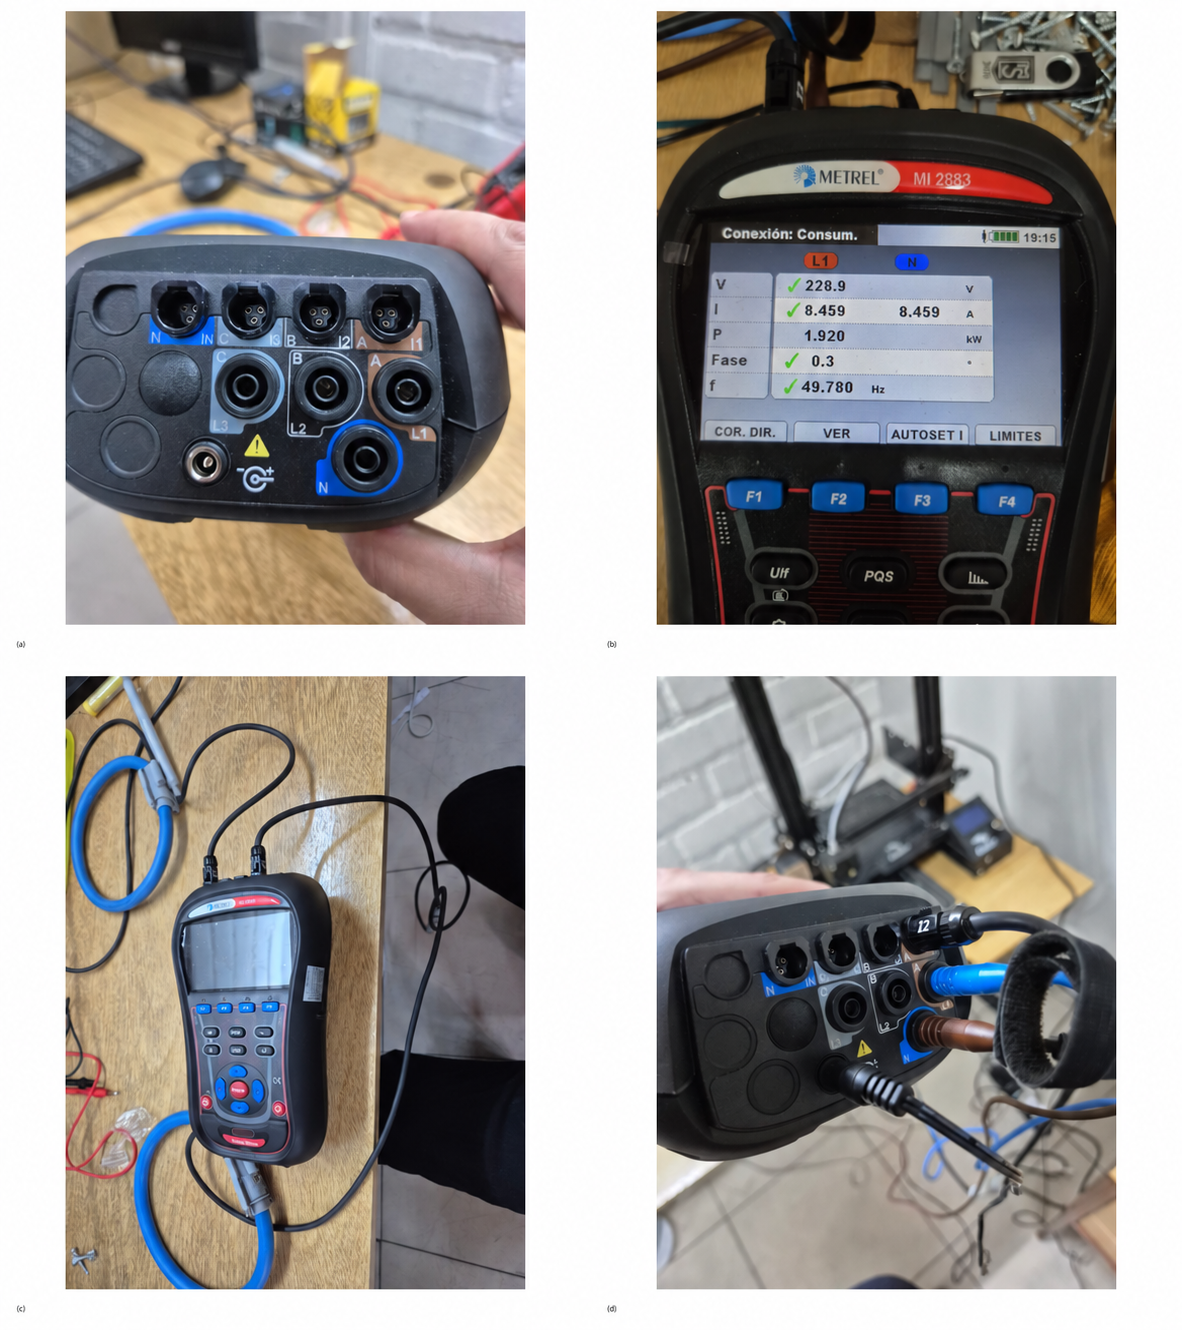
\includegraphics[width=0.91\textwidth]{figures/metrel_mi2883_photographic_record_updated.png}
\caption{Photographic record of the Metrel MI2883 used for the controlled single-phase EnPi comparison: (a) voltage and current input terminals; (b) instrument display during the campaign; (c) connected voltage leads and current-probe input; and (d) instrument and flexible current probe in the laboratory, including its calibration-identification label. The instrument was calibrated and certified by the Center for Instrumentation and Electronic Development (CIDE), Universidad de Santiago de Chile, under certificate CCE:814-2025 dated 20 October 2025.}
\label{fig:metrel-photographic-record}
\end{figure*}

The Metrel MI2883 was calibrated and certified by the Center for Instrumentation and Electronic Development (CIDE), Universidad de Santiago de Chile, on 20 October 2025 under certificate CCE:814-2025. The objective was to quantify the agreement between measurements obtained by EnPi and the reference instrument under controlled electrical-load scenarios. The experimental evidence comprises two distinct datasets: (i) a main campaign of ten scenarios (000--009) used to compare voltage, current, frequency, power factor, direct active power, and interval energy; and (ii) a separate 17-day industrial dataset used to demonstrate the measurement-to-EnPi workflow.

\begin{table}[!h]
\caption{EnPi--Metrel characterization scenarios and temporally paired observations.}
\label{tab:escenarios-reales-de-validacion-de-enpi-metre}
\centering
\begin{adjustbox}{max width=\columnwidth}
\begin{tabular}{p{0.1\textwidth}p{0.35\textwidth}p{0.1\textwidth}}
\toprule
Scenario & Description & Samples \\
\midrule
000 & No load (test 1) & 577 \\
001 & Light bulb & 1202 \\
002 & Laptop charging & 1191 \\
003 & Heater & 900 \\
004 & Mobile phone charging & 1201 \\
005 & Angle grinder & 1201 \\
006 & Monitor & 1201 \\
007 & Mixed: heater + mobile phone + laptop + light bulb & 1181 \\
008 & No load (test 2) & 900 \\
009 & Heater with power variations & 1042 \\
\bottomrule
\end{tabular}
\end{adjustbox}
\end{table}

These datasets are analyzed separately and are not treated as one homogeneous experiment.
The main campaign considered 10 single-phase load scenarios, including no-load, resistive, electronic, inductive, mixed-load, and periodic on/off conditions. In each scenario, both instruments measured the same load circuit simultaneously, with the EnPi current sensor and the Metrel clamps on the same phase conductor. Measurements were temporally paired by timestamp rounded to the second. Consequently, the 10,596 paired observations represent repeated time-series measurements nested within ten experimental scenarios, rather than 10,596 statistically independent experimental replications.

The EnPi node measures voltage, current, active power, accumulated energy, frequency, and power factor, and sends the readings to a remote data service along with a timestamp, meter code, and other origin metadata. The metering device consisted of a PZEM-004T TTL Modbus-RTU single-phase 100 A module, interfaced to the firmware via the \texttt{PZEM004Tv30} library. Based on the commercial data sheet for procurement, this variant has a nominal operating voltage and current range of 80--260 VAC and 0--100 A, respectively, with a frequency range of 45--65 Hz and a power factor of 0--1. The unit was housed in a single-phase measurement enclosure: the live wire supplying the monitored load connected to the single-phase conductor passing through the internal metering point, while the internal terminal blocks mated male and female plugs to sandwich the node between the grid and the load via an intermediary metering assembly. This arrangement does not alone confer electrical-safety compliance. 
An ESP32S3 firmware branch with NTP time synchronization and direct HTTPS delivery to the server was used for the transmission. The PCB implementation in Section~\ref{sec:hardware-reproducibility} supports hardware reproducibility, not a demonstration of electrical safety certification or regulatory conformance. The experimental logs for temporal pairing contain roughly 1-s timestamp spacing. The \texttt{payload\_raw} field contains the reading sent from the ESP32S3 and is stored without any intermediate backend processing. The EnPi archive also includes a measurement timestamp (\texttt{fecha\_hora}), a persistence timestamp (\texttt{created\_at}), and the original JSON payload. The two timestamp fields were retrospectively audited as they were recorded, with no timezone conversion applied. For 50,620 EnPi records, the difference \texttt{created\_at} minus \texttt{fecha\_hora} ranged from $-3600$ to $-2958$~s (median $-3592$~s). This is consistent with a nominal one-hour offset plus a variable residual but does not point to any specific time zone conversion or network latency. Thus, \texttt{created\_at} was not used to replace the measurement timestamp. Comparative metrics are based on the archived paired observations; missing observations were not interpolated.

The Metrel export retained the direct \texttt{P1+(Med) [W]} and interval-energy \texttt{Ep1+(Med) [mWh]} channels for the tests being monitored. EnPi and Metrel entries were matched by scenario and timestamp. Only records with a valid temporal counterpart were included in the pointwise agreement metrics; no observations were reconstructed. For the direct-power statistics, we used synchronized measurements with valid readings from both instruments. We did not remove any load observations for the per cent metrics, as the denominators are close to zero and do not allow meaningful interpretation of the relative errors; we also divided the EnPi power by 1000 to convert from kW to W. We computed accumulated energy only from timestamp-matched observations. In case that a gap disrupted the nominal one-second series, the scenario was divided into contiguous subsequences. We summed Metrel interval-energy quantities up to the retained matched observations and computed the EnPi accumulated-register change using the first and last observation of each contiguous sub-interval, then summed the partial values. 
This segment-matching technique prevents intervals with no matched EnPi observations from spanning intervals with unknown EnPi observations; items were neither interpolated nor reconstructed. 


\section{Results: Experimental Characterization Against the Metrel MI2883}
\label{sec:metrel-validation}
This section presents experimental characterization of the EnPi node using a Metrel MI2883 power quality analyzer. We conducted a controlled comparison campaign in 2026 using a Metrel MI2883 calibrated and certified by the Center for Instrumentation and Electronic Development (CIDE), Universidad de Santiago de Chile, on 20 October 2025 (certificate CCE:814-2025). We used the calibrated Metrel as the reference and evaluated EnPi as an IoT energy-monitoring sensor in controlled single-phase tests. The results show that the two instruments agreed under these test conditions. They do not certify EnPi’s metrological performance or demonstrate that the platform has been fully validated for industrial use.
For the primary campaign, 10 load cases and 10,596 time-matched observations were used. We aligned the records by scenario, truncated timestamps to the second, removed interrupted matches, and discarded unmatching timestamps before we computed pointwise errors. A continuity test on EnPi highlighted 15 discontinuities throughout the scenarios along with 210 one-second EnPi points and the associated baseline-instrument measurements. The gaps were 20 seconds in 000, 10s in 002, and 20s in 007, while they lasted 160s in 009. In Case 009, we split the 160 s into ten 1202-s during a 1202-s observation interval, in 10-30 s intervals. This left 1042 records that had matching timestamps.
These disconnections are the result of focal breaks in the data-acquisition chain and not measurement errors; we did not interpolate values over gaps in data. After identifying the issue, we created a firmware branch that stores readings that could not be transmitted and dumps them into the queue, then transmits them in chronological order once connectivity is reestablished. We mention this modification for reproducibility; it didn't help on the dataset in the experiment.  

\subsection{Metrics and Comparison Criteria}
\label{subsec:metrics-criteria}
We evaluated the results with MAE, RMSE, MAPE, WMAPE, mean bias, Pearson correlation, coefficient of determination (R2) and Bland–Altman LOA. MAE provides the magnitude of the error in the same units as the original measurement, while RMSE tends to penalize larger errors more. MAPE denotes relative error only when the reference value is physically meaningful. Bland–Altman analysis, on the other hand, quantifies agreement via the differences between techniques as opposed to their correlation alone \cite{r2_bland}.
To account for this bias in interpreting percent-based metrics, we considered only the reference values above the bottom limit. For active power, we adopted a different threshold for the normalized \texttt{P1+(Med)} channel since its values were expressed in kW. That threshold was. On the other hand, when analyzing the detection floor, we kept all values below that threshold, but not as evidence of accuracy proportional to the power of the detected signal line. For no-load situations and items with zero or near-zero reference readings, MAPE and WMAPE are labeled not applicable, or those MAPE and WMAPE values should be viewed only as boundary-case diagnostics; industrial performance quality should not be evaluated based on them.
We tested the results against operational acceptability criteria, rather than metrological certification classes. These specifications were based on three sources: manufacturer specifications for low-cost PZEM modules, IoT literature findings claiming PZEM-based monitors can measure close to commercial devices, and IEC standards for energy meter error limits as a rule of thumb. This is a comparison, but not for implying certification or regulatory compliance \cite{ref24}, \cite{ref25}. 

\paragraph{Metric definitions and pooling convention.}
For each valid paired observation $i$, let $P_i^{\mathrm{E}}$ denote EnPi active power in W, $P_i^{\mathrm{M}}$ the corresponding Metrel direct active-power measurement in W, and $e_i=P_i^{\mathrm{E}}-P_i^{\mathrm{M}}$. For a specified eligible set $\mathcal I$ of $n$ observations, the reported absolute-error, squared-error, and signed-error summaries are defined as
\begin{equation}
\mathrm{MAE}=\frac{1}{n}\sum_{i\in\mathcal I}|e_i|,\qquad
\mathrm{RMSE}=\sqrt{\frac{1}{n}\sum_{i\in\mathcal I}e_i^2},\qquad
\mathrm{Bias}=\frac{1}{n}\sum_{i\in\mathcal I}e_i.
\label{eq:r2_absolute_metrics}
\end{equation}
For positive and physically meaningful reference-power denominators, percentage errors are defined by
\begin{equation}
\mathrm{MAPE}=\frac{100}{n}\sum_{i\in\mathcal I}\frac{|e_i|}{|P_i^{\mathrm{M}}|},\qquad
\mathrm{WMAPE}=100\frac{\sum_{i\in\mathcal I}|e_i|}{\sum_{i\in\mathcal I}|P_i^{\mathrm{M}}|}.
\label{eq:r2_percentage_metrics}
\end{equation}
The pooled statistics reported are observation–weighted statistics over all the eligible loaded records, not the arithmetic means of the statistics computed at the scenario-level. Scenario 008 offers no valid direct-power pairs, and scenario 000 is not tested in the loaded pooled summary. The percentage calculations are excluded for zero-reference observations. A later local computational audit of the archived 9,119 valid loaded pairs derived MAPE = 3.86089760\% and WMAPE = 1.77307101\% as defined therein. The audit verifies the arithmetic of the already-filtered pair, but it does not define upstream raw-timestamp matching, nor does it derive a metrological uncertainty budget.

Therefore, the conditions in Tab.~\ref{tab:criterios-operacionales} are selection rules for operational monitoring rather than regulatory tolerances. They were established to determine whether the node was stable enough to enable EnPI determination, load-profile interpretation, and alert-priority analysis in the tested single-phase environment. These limits blend physical interpretability, the acquisition module's nominal operating range, the magnitude of the observed error relative to the comparison analyzer, and the flowchart's decision use. They should not be used for billing, certification, protection studies, or high-accuracy energy balances without a separate calibration and validation campaign. 

Supplementary Table S3 summarizes the reproducibility elements for the EnPi node, firmware identifier, payload provenance, temporal pairing, and repository structure. Supplementary Algorithm S1 and Supplementary Fig. S7 document the local buffering and retransmission logic implemented after the validation campaign.

\begin{table}
\caption{Operational acceptance criteria used to interpret the EnPi--Metrel comparison. These thresholds do not constitute metrological certification.}
\label{tab:criterios-operacionales}
\centering
\scriptsize
\begin{adjustbox}{max width=0.9\columnwidth}
\begin{tabular}{p{0.2\columnwidth}p{0.25\columnwidth}p{0.45\columnwidth}}
\toprule
Variable & Operational criterion & Justification \\
\midrule
Voltage & MAE $<$ 2 V & Operational screen for 220--230 V single-phase networks: the threshold is below 1\% of nominal voltage and is applied to relevant supply deviations, not to certify meter class.  \\
Current under load & MAPE $<$ 10\% and joint review with MAE & The percentage error only gives useful information when the denominator makes sense in real-world terms, and MAE is preferred at low or near-zero current to prevent large relative errors. \\
Frequency & MAE $<$ 0.1 Hz & Absolute deviations are not energy-relevant but can affect correlation.: Used as an operational stability criterion since the grid frequency oscillates within a small range; however, small absolute deviations can influence the correlation. and thus do not affect the decisions of the energy management. \\
Power factor & MAE $<$ 0.03 & It can distinguish general resistive, inductive, electronic, or combined profiles with a good level of accuracy; however, it is not applicable for billing or regulatory purposes.  \\
Active power, main campaign & Direct MAE, RMSE, bias, MAPE, WMAPE, and agreement & Compared with the Metrel \texttt{P1+(Med)} channel, only synchronized, valid readings are included. No-load tests indicate the detection limit; they do not measure proportional accuracy.\\
Accumulated energy & Scenario-level segment-matched difference & The Metrel interval-energy values were added over timestamp-matched observations and compared to the EnPi register changes that were computed separately for each contiguous one-second interval.
\\
\bottomrule
\end{tabular}
\end{adjustbox}
\end{table}

\begin{table*}
\caption{Scenario-level error for variables directly measured against the Metrel MI2883. N/A indicates no-load scenarios or zero/near-zero reference denominators, where percentage metrics have no robust physical interpretation and absolute-error metrics should be prioritized. Current is expressed in A and frequency in Hz.}
\label{tab:error-por-escenario-para-variables-medidas-di}
\centering
\scriptsize
\begin{adjustbox}{max width=0.8\textwidth}
\begin{tabular}{cccccccccc}
\toprule
Sc. & n & MAE V & MAPE V & MAE I & MAPE I & MAE f & MAPE f & MAE PF & MAPE PF \\
\midrule
000 & 577 & 0.832 & N/A & N/A & N/A & 0.047 & 0.09\% & N/A & N/A \\
001 & 1202 & 0.832 & 0.36\% & 0.011 & 3.94\% & 0.042 & 0.08\% & 0.0107 & 1.09\% \\
002 & 1191 & 0.840 & 0.37\% & 0.011 & 3.41\% & 0.047 & 0.09\% & 0.0093 & 1.93\% \\
003 & 900 & 0.840 & 0.37\% & 0.134 & 1.65\% & 0.069 & 0.14\% & 0.0030 & 0.30\% \\
004 & 1201 & 0.853 & 0.37\% & 0.012 & 7.80\% & 0.071 & 0.14\% & N/A & N/A \\
005 & 1201 & 0.945 & 0.41\% & 0.056 & 3.75\% & 0.066 & 0.13\% & 0.0017 & 0.17\% \\
006 & 1201 & 0.927 & 0.40\% & 0.012 & 3.37\% & 0.054 & 0.11\% & 0.0126 & 2.29\% \\
007 & 1181 & 0.940 & 0.41\% & 0.167 & 1.95\% & 0.046 & 0.09\% & 0.0006 & 0.07\% \\
008 & 900 & 1.034 & 0.45\% & 0.043 & N/A & 0.069 & 0.14\% & N/A & N/A \\
009 & 1042 & 0.922 & 0.40\% & 0.127 & 2.45\% & 0.052 & 0.10\% & 0.0039 & 0.40\% \\
\bottomrule
\end{tabular}
\end{adjustbox}
\end{table*}

The scenario-level MAPE heat map is provided in Supplementary Fig. S5. The scenario-wise MAE and MAPE were recomputed from finite paired EnPi--Metrel readings using $\mathrm{MAE}=n^{-1}\sum_i|E_i-M_i|$ and $\mathrm{MAPE}=100n^{-1}\sum_i|E_i-M_i|/|M_i|$ for nonzero reference readings. MAPE is not reported for the unloaded scenarios where the denominator or device detection threshold makes a relative percentage physically misleading (including current in scenario 008); absolute errors are retained where interpretable. No post-hoc outlier exclusion was applied. The physical origin of low-current offsets has not been established.
The scenario-level error results show that voltage remains stable in the operating scenarios, with MAPE below 0.50\% for scenarios 001--009 and larger boundary-case deviation only in the first no-load test. This indicates that EnPi voltage measurement is consistent for operational monitoring in the tested 220--230 V single-phase networks. For current, relative error increases at low loads, especially for mobile phone charging and no-load/standby-like conditions, where MAE is low in absolute terms, but the reference denominator is also small. Therefore, we separate the interpretation into no-load or low-load conditions, where MAE and detection-floor behavior are more informative, and productive or thermal-load conditions, where MAPE enables proportional error comparison.

\begin{table*}
\caption{Global correlation and Bland-Altman agreement between EnPi and Metrel MI2883.}
\label{tab:correlacion-global-y-acuerdo-de-bland-altman-}
\centering
\scriptsize
\begin{adjustbox}{max width=0.8\textwidth}
\begin{tabular}{ccccccc}
\toprule
Variable & Pearson r & R\textasciicircum{}2 & Bias & SD & Lower LoA & Upper LoA \\
\midrule
Voltage & 0.9840 & 0.9682 & 0.8947 & 0.2994 & 0.3079 & 1.4815 \\
Current & 0.9998 & 0.9997 & -0.0589 & 0.0835 & -0.2225 & 0.1048 \\
Frequency & 0.8255 & 0.6815 & -0.0408 & 0.0531 & -0.1450 & 0.0633 \\
Power factor & 0.9968 & 0.9937 & -0.0015 & 0.0181 & -0.0370 & 0.0341 \\
\bottomrule
\end{tabular}
\end{adjustbox}
\end{table*}

Current and power-factor scatter plots are shown in the Supplementary Fig. S6. The scatter-plot analysis tests whether the system is proportional to the reference instrument (Supplementary Fig. S6). The current is close to a linear fit, consistent with $r=0.9998$ and $R^2=0.9997$. This observation has to be interpreted together with absolute errors and limits of agreement; a large correlation alone is not indicative of metrological agreement. The power factor shows a very good fit overall; however, the Bland-Altman scatter is largely biased by a small number of extreme paired differences in scenario 002 (r=0.9968; R2=0.9937). As a consequence, use it for general load-profile analysis cautiously, especially when readings are transient or abnormal.

\begin{figure*}
\centering
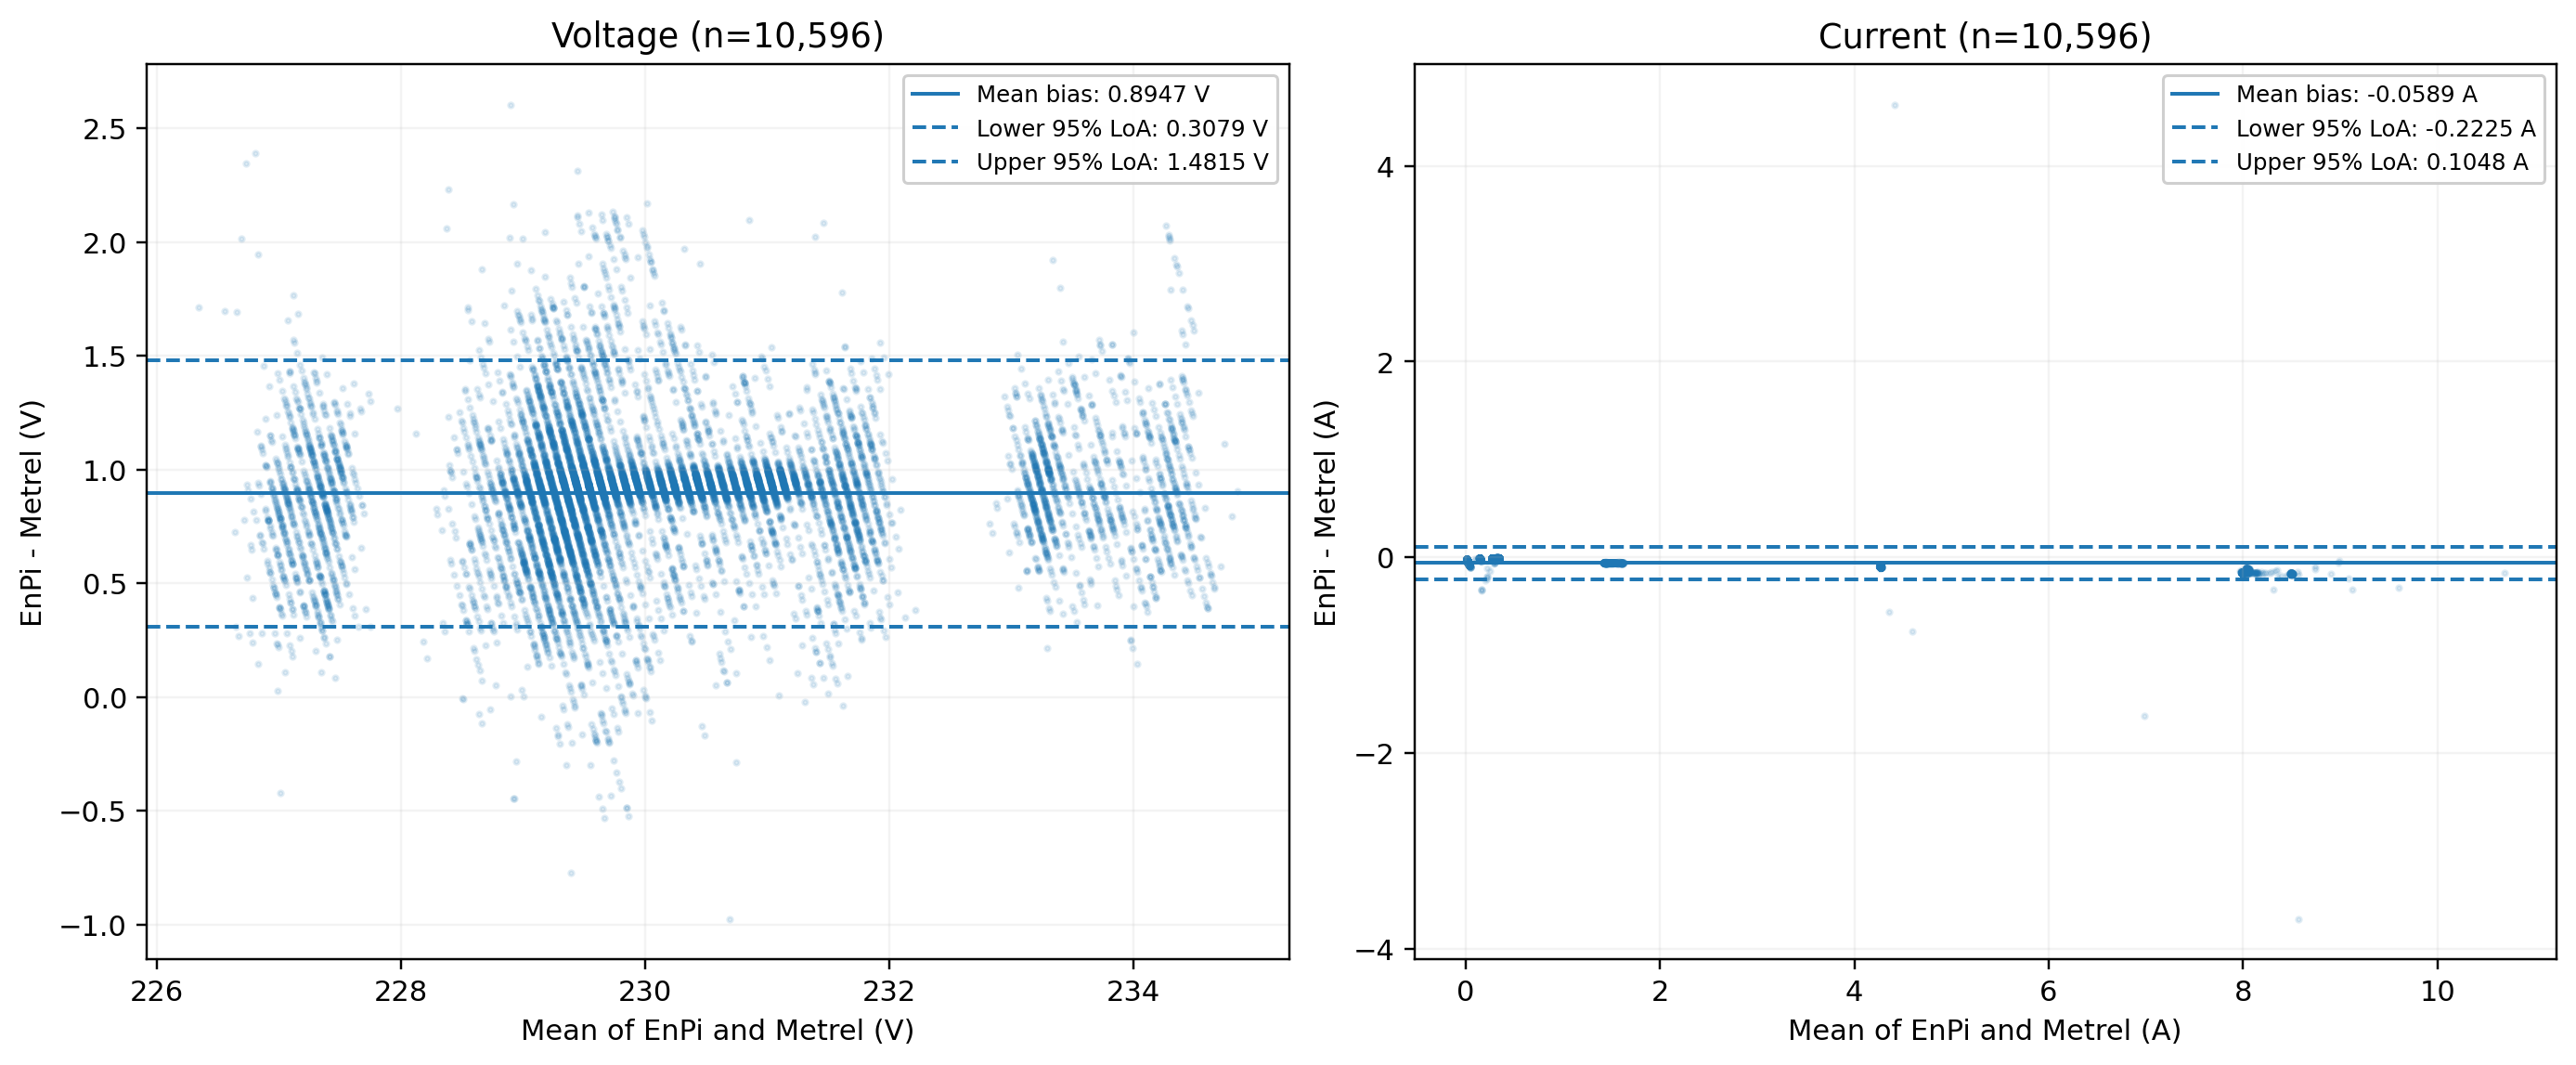
\includegraphics[width=0.98\textwidth,trim=45 35 45 35,clip]{figures/image11.png}
\caption{Bland--Altman analysis reconstructed from 10,596 paired observations for voltage and current (EnPi minus Metrel). Horizontal lines show the mean bias and descriptive 95\% limits of agreement (mean $\pm$ 1.96 sample standard deviations).}
\label{fig:10}
\end{figure*}

Figure~\ref{fig:10} shows agreement in physical units, along with the correlations. Voltage has an average bias of approximately 0.895 V, with limits of agreement of 0.308 V and 1.481 V. This small, systematic difference may indicate an instrument offset and could be compensated by a secondary calibration if higher accuracy is required. The average current bias is -0.0589 A, with limits of -0.2225 A to 0.1048 A, indicating EnPi tends to read slightly lower than Metrel for current. Whether this degree of error is acceptable is application-specific; the limits of agreement do not determine that. Some additional verification would be necessary to justify the use of measurements for high-accuracy energy balances. Because the Metrel output provided active power, it was directly comparable rather than derived from voltage, current, and power factor. The analysis was performed using time-synchronized data from both instruments. We included no-load measurements to gauge the detection floor, but we did not interpret their MAPE. 

\begin{table*}[!htbp]
\caption{Direct active-power comparison using the Metrel \texttt{P1+(Med)} channel. Errors are calculated as EnPi minus Metrel. Scenario 008 has no valid numerical reference-power pairs and is excluded from direct-power accuracy statistics.}
\label{tab:direct-power-main}
\centering
\scriptsize
\setlength{\tabcolsep}{4pt}
\begin{adjustbox}{max width=0.94\textwidth}
\begin{tabular}{ccccccc}
\toprule
Scenario & Paired observations & MAE (W) & RMSE (W) & Bias (W) & MAPE (\%) & WMAPE (\%) \\
\midrule
000 & 575 & 0.769 & 0.836 & $-0.769$ & N/A & N/A \\
001 & 1202 & 1.677 & 1.862 & $-1.677$ & 2.660 & 2.661 \\
002 & 1191 & 1.465 & 3.034 & $-1.296$ & 4.034 & 4.035 \\
003 & 900 & 23.889 & 24.080 & $-23.889$ & 1.307 & 1.307 \\
004 & 1201 & 1.777 & 1.780 & $-1.777$ & 9.807 & 9.808 \\
005 & 1201 & 9.831 & 9.839 & $-9.831$ & 2.936 & 2.934 \\
006 & 1201 & 2.279 & 2.282 & $-2.279$ & 5.215 & 5.215 \\
007 & 1181 & 30.972 & 30.984 & $-30.972$ & 1.589 & 1.589 \\
008 & 0 & N/A & N/A & N/A & N/A & N/A \\
009 & 1042 & 24.481 & 54.584 & $-21.402$ & 2.481 & 1.926 \\
Loaded pooled & 9119 & 11.408 & 23.184 & $-11.034$ & 3.861 & 1.773 \\
\bottomrule
\end{tabular}
\end{adjustbox}
\end{table*}

Across the nonzero-load scenarios with a valid direct-power reference, the pooled Pearson correlation was 0.9998 ($R^2=0.9996$). The mean bias was $-11.03$ W, with a pooled MAE of 11.41 W and a pooled MAPE of 3.86\%. The magnitude-dependent scenario results are more informative than the pooled MAE alone. Errors of approximately 24--31 W in the higher-power scenarios 003, 007, and 009 corresponded to MAPE values of only 1.31--2.48\%, whereas scenario 004 had a 1.78 W MAE but a 9.81\% MAPE because its reference power was only approximately 18 W. This behavior is expected when relative-error metrics are applied to small denominators and does not represent the operating condition for which the node is intended to support industrial EnPI monitoring.

Scenario 008 is retained as a documented boundary scenario, but the source reference-power channel does not provide valid numerical observations for direct-power comparison. Accordingly, its MAE, RMSE, and bias are not estimable and are reported as N/A. No-load behavior must be characterized in a separate acquisition with a valid reference channel.

\begin{table*}[!htbp]
\caption{Accumulated-energy comparison using only timestamp-matched observations. Gaps split each scenario into contiguous one-second segments. Metrel energy is the sum of retained interval-energy observations; EnPi energy is the sum of accumulated-register changes calculated separately within the same segments.}
\label{tab:energy-direct-main}
\centering
\scriptsize
\setlength{\tabcolsep}{4pt}
\begin{adjustbox}{max width=0.86\textwidth}
\begin{tabular}{cccccc}
\toprule
Scenario & Matched observations & Contiguous segments & Metrel energy (Wh) & EnPi change (Wh) & Difference (\%) \\
\midrule
000 & 577 & 3 & 0.123 & 0.000 & N/A (below resolution) \\
001 & 1202 & 1 & 21.045 & 20.996 & $-0.235$ \\
002 & 1191 & 2 & 12.010 & 11.002 & $-8.397$ \\
003 & 900 & 1 & 456.971 & 451.996 & $-1.089$ \\
004 & 1201 & 1 & 6.044 & 5.997 & $-0.772$ \\
005 & 1201 & 1 & 111.816 & 108.993 & $-2.525$ \\
006 & 1201 & 1 & 14.582 & 14.000 & $-3.991$ \\
007 & 1181 & 3 & 639.345 & 630.012 & $-1.460$ \\
008 & 900 & 1 & 0.000 & 0.000 & N/A (no load) \\
009 & 1042 & 11 & 367.947 & 361.023 & $-1.882$ \\
\bottomrule
\end{tabular}
\end{adjustbox}
\end{table*}

The segment-matched energy comparison yields differences ranging from $-8.397\%$ (scenario 002) to $-0.235\%$ (scenario 001) among the nonzero scenarios. Scenarios 002, 007, and 009 contain 2, 3, and 11 contiguous segments, respectively. Calculating the EnPi register change separately within each segment prevents its counter from spanning unmatched intervals; the Metrel total is likewise restricted to the retained timestamp-matched observations. In scenario 009, this criterion uses 1042 matched observations and yields a difference of $-1.882\%$. The effective 1 Wh EnPi register resolution can substantially influence short, low-energy tests; consequently, the results characterize the tested scenarios but do not constitute certified energy-accuracy specifications.

\subsection{Segment-Preserving Bootstrap Sensitivity Analysis}
\label{subsec:bootstrap-r2}
A circular moving-block bootstrap was used within each contiguous valid segment to describe sampling variability without assuming that temporally adjacent observations were independent. 
The procedure preserved scenario and gap boundaries, used 2000 replicates, and examined block lengths of 15, 30, 60, and 120 observations. For the primary 60-observation block length, the conditional 95\% percentile intervals were 11.054--11.959 W for pooled MAE, 15.926--32.697 W for RMSE, $-11.207$ to $-10.822$ W for bias, and 1.718--1.854\% for WMAPE.
The observed pooled estimates were 11.408 W, 23.184 W, -11.034 W, and 1.773\%, respectively. The RMSE bounds were more strongly influenced by the large-error observations. For block lengths $L=15,30,60,120$, the lower and upper percentile boundaries were 11.054--11.066 and 11.939--12.014 W for MAE; 15.916--15.982 and 32.451--33.253 W for RMSE; $-11.245$--$-11.187$ and $-10.858$--$-10.771$ W for bias; and 1.718--1.721 and 1.847--1.869\% for WMAPE. These are descriptive ranges of interval endpoints across block-length choices, not additional confidence intervals or evidence of device-to-device generalizability. Percentage-error metrics require additional caution near zero reference power, where the denominator can make relative error unstable \cite{r2_hyndman}. These are conditional intervals and do not address uncertainty across scenarios and groups of scenarios in the form of independently manufactured devices or days or reference instrument. Each repeat draws blocks with a fixed length from within the same contiguous window of scenario segments, limits the concatenated resample to the length of the original segment, and then combines the re-sampled contributions across segments before calculating pooled metrics. The stored executable implementation was run again on the 91,119 already-aligned observations (NumPy default\_rng seed $20261013+L$ for each block length), re-deriving the reported 60-observation intervals to the presented rounding. This computational reproduction does not validate one-step upstream alignment of raw device and reference timestamps. The specified block length in step 2.3 can be written as a function of the data length n and t. The stationary bootstrap of Politis and Romano \cite{r2_politis} can be viewed as a beacon of background information, but it uses random rather than fixed block lengths and is not the algorithm used in this work. Circular wrapping is a computational trick at section edges, and neither methodology substitutes for a metrological uncertainty budget \cite{r2_gum}. 

\section{Hardware Reproducibility}
\label{sec:hardware-reproducibility}
We implemented the sensing-node carrier as a custom PCB to improve wiring consistency and make the prototype reproducible beyond a breadboard or ad hoc assembly. Figure~\ref {fig: pcb-implementation} shows the PCB top and bottom views, and Figure~\ref{fig: pcb-schematic-main} provides the full electrical schematic at full manuscript width. The PCB includes the ESP32-S3-WROOM-1 communication unit, a USB-C programming and power interface, the external UART connector for the PZEM-004T single-phase metering module, an isolated HLK-PM01 AC--DC supply, an AP2112K-3.3 voltage regulator, reset and boot buttons, fused mains input, AC pass-through terminals, and a MAX3485 RS485 transceiver with termination components. This PCB is the hardware carrier for the single-phase sensing node under test. In the working acquisition path for single-phase measurement, we used the PZEM-004T interface in the experimental campaign. An RS485 expansion port was added to connect to industrial meters or three-phase measurement units, but three-phase operation is not tested in this paper. This distinction matters: the PCB adds extensibility and manufacturability, and the performance claims in Section~\ref{sec:metrel-validation} apply only to the single-phase, tested PZEM-based configuration. Table~\ref{tab:pcb-component-summary} summarizes the main components, and Supplementary Table S4 provides the complete bill of materials to preserve manuscript readability and reproducibility. 

\begin{table}[H]
\caption{Compact hardware summary of the implemented EnPi PCB. The complete BOM is provided as Supplementary Table S4.}
\label{tab:pcb-component-summary}
\centering
\scriptsize
\begin{adjustbox}{max width=0.94\columnwidth}
\begin{tabular}{p{0.32\columnwidth}p{0.58\columnwidth}}
\toprule
Function & Implemented element \\
\midrule
Processing and communication & ESP32-S3-WROOM-1 module with firmware-controlled acquisition and transmission \\
Single-phase metering interface & External UART connector for the PZEM-004T metering module validated in this study \\
Industrial-meter expansion & MAX3485 RS485 transceiver with selectable termination for future meter integration \\
Power stage & HLK-PM01 AC--DC supply and AP2112K-3.3 voltage regulator \\
Installation and protection & Fused mains input, AC pass-through terminal blocks, and service-accessible reset/boot controls \\
Programming and service & USB-C connector for programming, maintenance, and local power during development \\
\bottomrule
\end{tabular}
\end{adjustbox}
\end{table}

\begin{figure*}[!t]
\centering
\begin{adjustbox}{max width=\textwidth}
\begin{tabular}{cc}
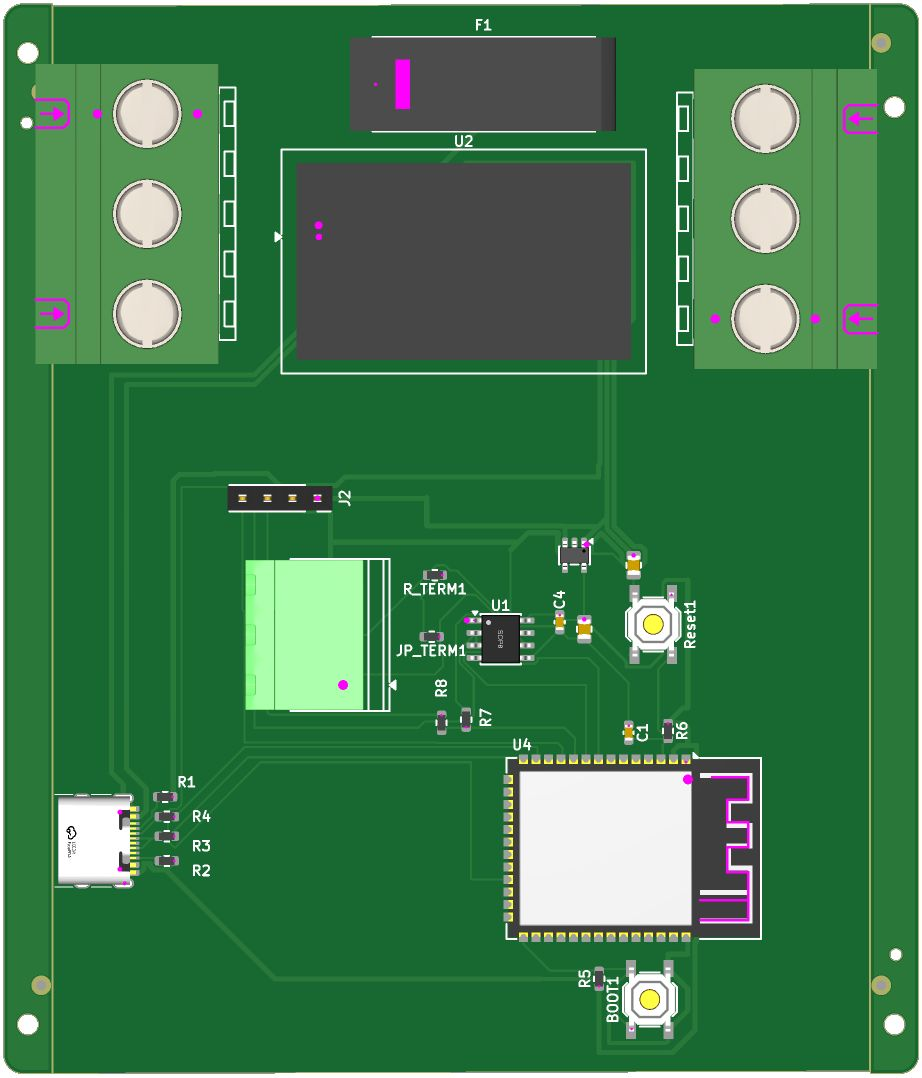
\includegraphics[width=0.43\textwidth]{figures/enpi_pcb_top.jpg} &
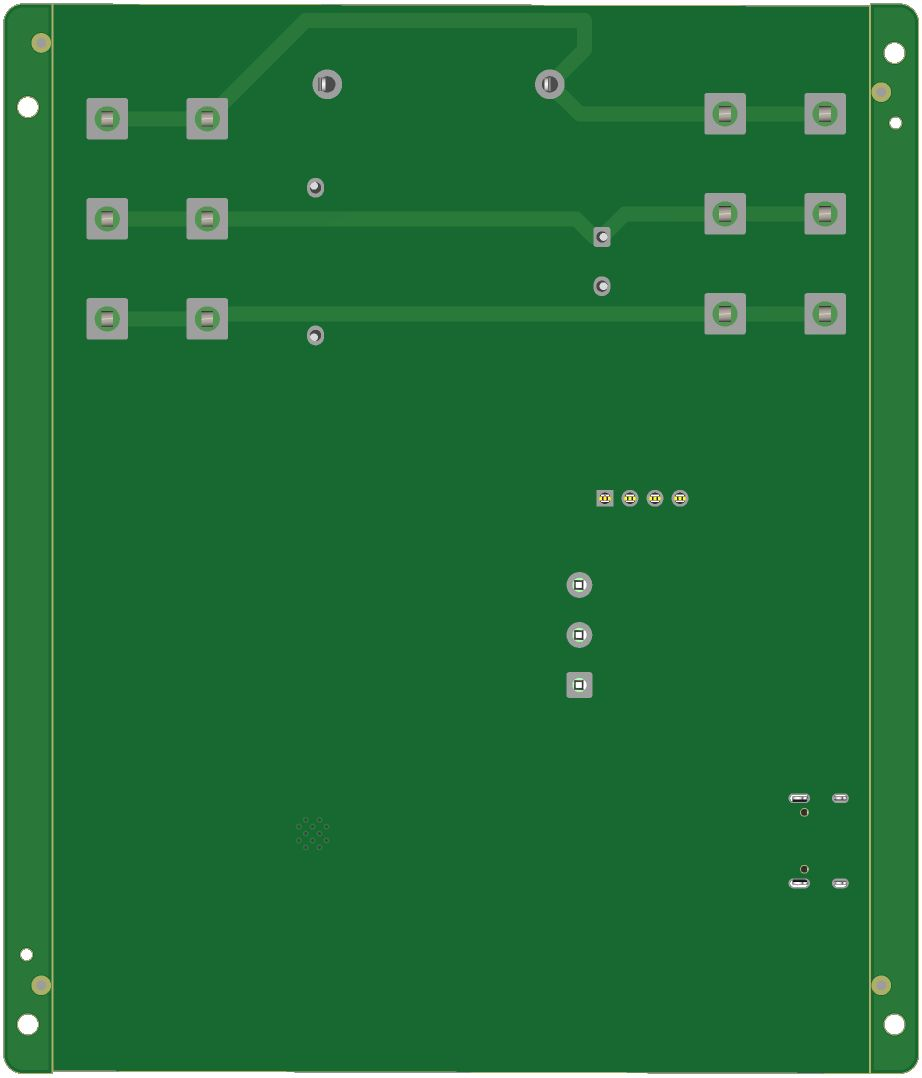
\includegraphics[width=0.43\textwidth]{figures/enpi_pcb_bottom.jpg} \\
(a) PCB top side & (b) PCB bottom side \\
\end{tabular}
\end{adjustbox}
\caption{We implemented the EnPi PCB, suitable for a low-cost sensing node, on the EnPi PCB used as the hardware platform. The validated path in this paper covers the single-phase PZEM-004T interface; the RS485 interface documents planned extensibility to other meters and future three-phase solutions, which will not be validated in the current campaign.}
\label{fig:pcb-implementation}
\end{figure*}

\begin{figure*}[!t]
\centering
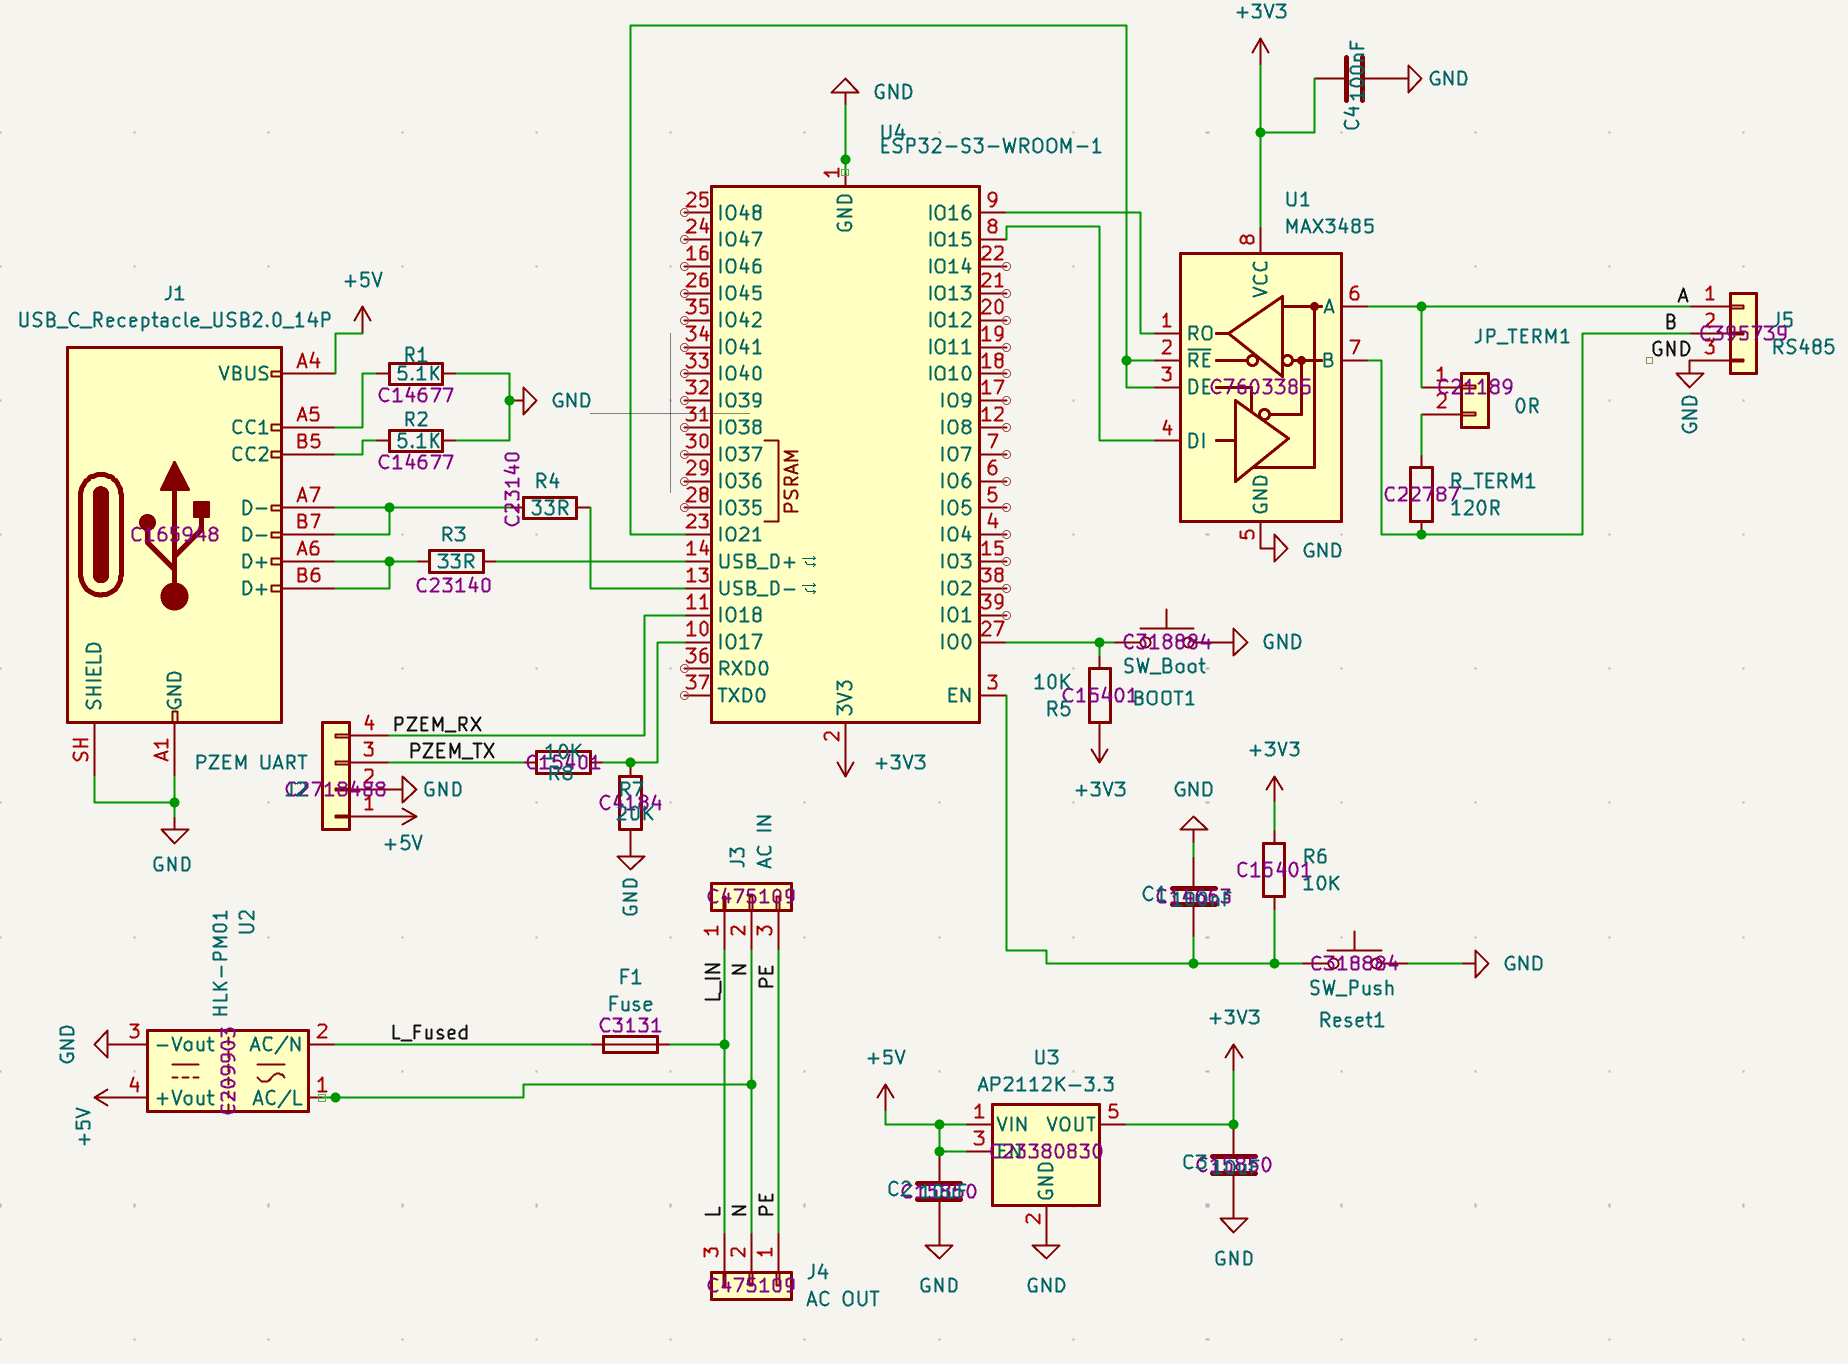
\includegraphics[width=0.98\textwidth]{figures/enpi_pcb_schematic.png}
\caption{Electrical schematic of the implemented EnPi PCB. The schematic supports hardware reproducibility and distinguishes the experimentally validated PZEM-004T single-phase measurement interface from the RS485 expansion path reserved for future three-phase or external-meter integration.}
\label{fig:pcb-schematic-main}
\end{figure*}

\section{Food-Sector Case Study: Platform Implementation and EnPI Traceability}
\label{sec:proposed-architecture}

\subsection{Platform Workflow Supporting the Case Study}
For the food-sector use case, the web platform serves as the workflow layer linking the characterized sensing node to production records and EnPI calculation. The web platform is not portrayed as an independently validated industrial SaaS platform. In this article, the web platform demonstrates how a low-cost node sends time-stamped electrical readings, how the readings retain source metadata, and how they link to production records to calculate EnPI at the machine level.
There are four main steps in the sensing workflow. First, it gathers the original data from the IoT node. Next, it links each record to relevant business information, such as the company, site, meter, equipment, reporting period, and data source. Following this, EnPI values are calculated using energy and production data for corresponding periods. Lastly, it adds the data source to each indicator, which helps in tracing back to the original measurement. Functional layers beyond those shown in the main text are listed in the online-only Supplementary Table S2. 

\begin{figure*}[t]
\centering
\begin{adjustbox}{max width=0.98\textwidth}
\begin{tikzpicture}[
    node distance=0.7cm and 0.8cm,
    block/.style={draw, rounded corners=2pt, align=center, minimum height=1.05cm, minimum width=2.85cm, font=\small},
    smallblock/.style={draw, rounded corners=2pt, align=center, minimum height=0.75cm, minimum width=2.55cm, font=\footnotesize},
    arrow/.style={-{Latex[length=2.2mm]}, thick}
]
\node[block, fill=gray!8] (load) {Single-phase\\machine/load};
\node[block, fill=blue!8, right=of load] (node) {Low-cost IoT\\sensing node};
\node[block, fill=blue!8, right=of node] (payload) {Raw payload\\timestamp\\meter ID};
\node[block, fill=green!8, right=of payload] (store) {Provenance-aware\\data service};
\node[block, fill=orange!10, right=of store] (enpi) {Machine-level\\EnPI};

\node[smallblock, fill=gray!8, below=of payload] (prod) {Production record\\compatible period};
\node[smallblock, fill=gray!8, above=of node] (ref) {Reference analyzer\\Metrel MI2883};
\node[smallblock, fill=orange!10, below=of enpi] (flags) {Reference value\\status flag\\audit trail};

\draw[arrow] (load) -- (node);
\draw[arrow] (node) -- (payload);
\draw[arrow] (payload) -- (store);
\draw[arrow] (store) -- (enpi);
\draw[arrow] (prod) -- (store);
\draw[arrow] (ref) -- node[midway, right, font=\footnotesize] {comparison} (node);
\draw[arrow] (enpi) -- (flags);
\end{tikzpicture}
\end{adjustbox}
\caption{
Sensor-to-indicator processing studied in this work. The experimentally characterized node collects single-phase electrical quantities, retains the raw payload and source metadata, and provides a provenance-aware data service that aligns measurements with compatible production records to enable machine-level EnPI calculation.}
\label{fig:sensor-to-indicator-workflow}
\end{figure*}

The process starts by gathering energy and production data from the available sources. Each record has metadata that describes its provenance — whether the source data was a manual input, a utility bill, an existing meter, or an IoT device. The platform links energy consumption to a specific operational unit and matches production, by time and duration, to the corresponding periods. This enables conversion of electricity readings into functional units of output such as energy per product, batch, shift, or machine.
In the IoT configuration considered in this work, the EnPi node is attached to a single-phase metering point, not the entire plant. This constrained deployment means the study's conclusions rest on what was actually tested: a sensing element with specific attributes and a reliable data path.
In addition, Supplementary Fig. S1 shows an alternative deployment scenario where nodes expansion and contextual alert generation are supported. Distributed metering provides time and space resolution, and the workflow preserves traceability while associating measurements with production data. This claim is only valid for single-phase sensing in the version of the tested technology and should not be interpreted as a complete industrial plant certification. Moreover, event-triggered notifications, associated devices, and predefined workflows are architectural enhancements, and this work does not empirically investigate them. 

\subsection{Traceable EnPI Data Model and Bounded Operational Demonstration}
\label{sec:enpi-data-model}
EnPI has the nature of analytical quality, as an energy performance indicator (EnPI) is an indicator that relates energy consumption to an energy-consuming parameter that has been identified. EnPI lets you see energy consumption as a function of product output, operating period, or business division, rather than monitoring only raw kWh. This matters because increased energy consumption is not necessarily energy degradation, and decreased energy consumption is not necessarily an improvement, unless you relate it to production level, shift, process, or operating environment.In summary, the indicator is defined as the energy consumed in the study period divided by the output of the process in the same period: 

\begin{equation}
\mathrm{EnPI}=\frac{\mathrm{Energy\ consumption\ (kWh)}}{\mathrm{Production}}
\label{eq:enpi}
\end{equation}

Production can be measured in terms of units produced, batches, tons, square meters, hours of operation, services rendered, or any other output measure relevant to the type of production and the business.

\begin{figure*}[!t]
\centering
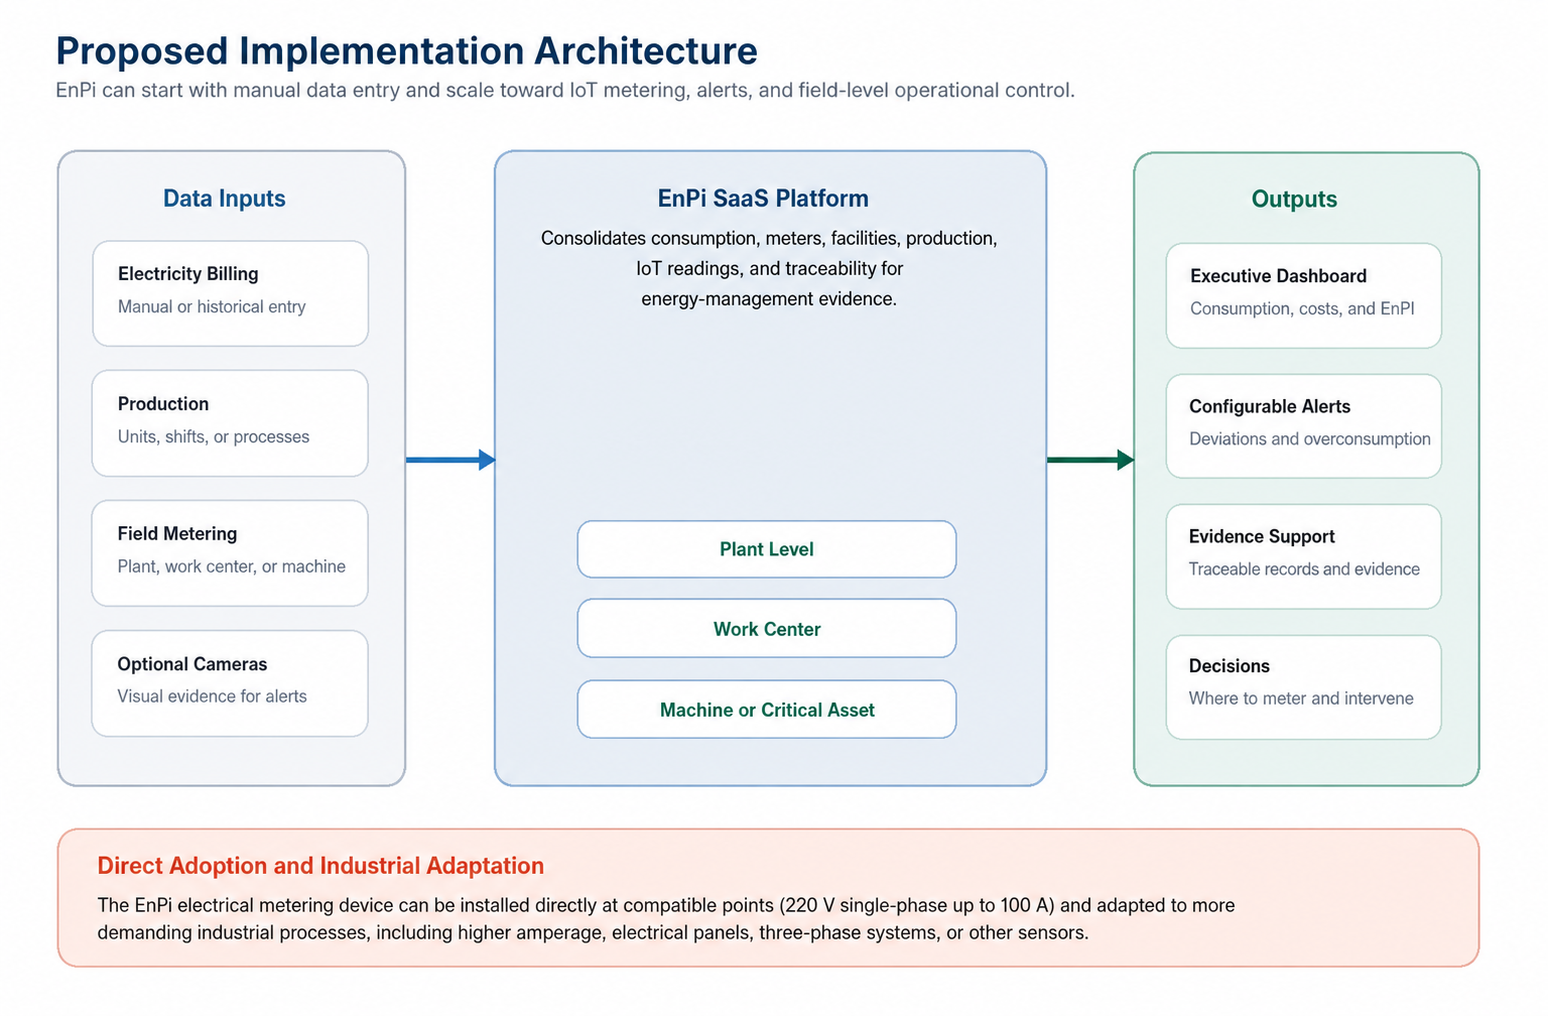
\includegraphics[width=0.9\textwidth]{figures/image1.png}
\caption{Conceptual EnPi data model for energy traceability, production, reconciliation, and energy performance indicators.}
\label{fig:data-model}
\end{figure*}

This indicator is only relevant if the underlying data are auditable. For an EnPI to be relevant, it needs to not only keep consumption and production data, but also relate them to a comparable time, data source, or operational unit, and to the individual or mechanism responsible for managing them. In energy management, this requirement is fulfilled by EnPI with a relational data model that contains business, building, meter, equipment, consumption, production, data source, target reference, reconciliation, and audit entities. The model retains the source of every record, differentiates between manual and IoT data, and shows how the data was generated.
The data model has three main sections. The first set of data relates to organizational and physical objects: company, building, work center, machine, meter, and IoT node. The second category of data is transactional entities that hold consumption records, IoT readings, production records, analysis periods, and data sources. Finally, the third group of data is analytical and governance entities: EnPI references, comparison rules, deviation states, source reconciliation, audit, and system parameters. A screen-level representation of the weekly production module is provided in the supplementary Fig. S2. 

\subsection{Anonymized Operational Traceability Case}
\label{subsec:real-enpi-case}

To make explicit the traceability chain the workflow seeks to preserve, we incorporated a bounded operational case from an anonymized food-sector SME. This case is used to demonstrate sensor-data provenance and EnPI calculation, not to validate industrial-scale performance or diagnose efficiency causes. The metering point corresponded to a single-phase dough sheeter used to process dough. During the 17-day monitoring period, the enterprise reported producing 44 kg of dough per day, based on its pre-established order schedule. The amounts per day were not separately weighed or checked. The total reported for the surveillance period was therefore 748 kg. The EnPi node sampled IoT measurements at a production rate for 17 production days from 31 July to 16 August 2026. This industrial demonstration is to be contrasted with the ten controlled EnPi--Metrel scenarios, which the project team attests were also performed in 2026 after the reference-instrument calibration date; the industrial period must not be taken to indicate the exact dates of the controlled comparison. Because we noticed a conversion problem in some processed columns, we rebuilt the electrical variables for this case from the \texttt{payload\_raw} field; therefore, we maintained the device-reported values. 

We estimated daily consumption as the difference between the last and first valid corrected cumulative-energy counter reading within each calendar day, and we calculated EnPI as kWh per kg of processed dough. The source workbook (\texttt{Lecturas Enpi\_V2.xlsx}, sheet \texttt{Lecturas Enpi}) has 19,982 time-stamped entries for meter \texttt{Amelie01} across 17 days. A separate local recomputation from the 19,982 stored readings yielded a sum of 17 intra-day counter increments of 17.986999 kWh (rounded to 17.987 kWh), while the counter difference observed in the first and last readings during the whole period was 18.094999 kWh (rounded to 18.095 kWh). The 0.108 kWh difference occurs at the transition from August 5 to 6, with the first counter reading on August 6 being greater than the last reading on August 5. The data do not explain what happened during this unmonitored period, and the intra-day amount does not account for it. Hence, the two sums represent differing
degrees of temporal coverage and therefore are not interchangeable. As a first-order operational baseline, the process flow assumed 0.0228 kWh/kg. This reference is not an official standard or certified target; it provides EnPi with an indication of observed performance relative to an operational baseline. Previous research in bakeries has shown that the ranges of kneading and other processes differ greatly depending on the type of product, size, equipment, and operation \cite{ref22}, \cite{ref23}. Over 17 production days, the sum of within-day increments was 17.987 kWh for a reported production of 748 kg, corresponding to a production-weighted EnPI of 0.0240468 kWh/kg (0.0240 kWh/kg). and a median daily EnPI of 0.0222045 kWh/kg (reported as 0.0222 kWh/kg). Different aggregation definitions for the two indicators; neither includes the 0.108 kWh inter-day increment that is not allocated to either indicator. According to the configured rule, 12 days were green, 1 day was warning, and 4 days were red. The red label was applied to August 4, August 7, August 10, and August 14, 2026 (deviations between +33.67\% and +59.99\% from the operational reference). The labels are operational flags based on rules, not automatically generated indicators of inefficiency. 

\begin{table}[H]
\caption{Summary of the anonymized 17-day EnPI traceability case in a food-sector SME dough sheeter.}
\label{tab:caso-real-summary}
\centering
\scriptsize
\begin{tabular}{p{0.55\columnwidth}p{0.35\columnwidth}}
\toprule
Metric & Value \\
\midrule
Operational period & 2026-07-31 to 2026-08-16 \\
Production days & 17 \\
Enterprise-declared production & 44 kg/day, based on the reported order schedule \\
Total production & 748 kg \\
Sum of observed within-day energy & 17.987 kWh \\
Full-period counter difference & 18.095 kWh \\
Inter-day unobserved counter increment & 0.108 kWh \\
Weighted EnPI & 0.0240 kWh/kg \\
Median daily EnPI & 0.0222 kWh/kg \\
Operational reference & 0.0228 kWh/kg \\
Minimum daily EnPI & 0.0173 kWh/kg \\
Maximum daily EnPI & 0.0365 kWh/kg \\
Status distribution & 12 green, 1 warning, 4 critical \\
\bottomrule
\end{tabular}
\end{table}

These variances meant the small business owner could think about the potential sources of abnormal energy intensity from all line items (i.e., number of dough pass, idle time, cleaning time, scheduling, etc.) or where effective machine loading might come from. The platform was not essentially infer the causes, but provide result of evidence to support user to focus and prioritize the operational diagnosis. The illustration below states that EnPi may be derived from raw data to operational decisions via a minimum chain: IoT read \texttt{payload\_raw}, physical variable conversion, estimation of daily energy, linkage to operational object, daily production reconciliation, calculation of EnPi, comparison against reference, visualization of dashboard, and registration of status. This enables the indicator to be traced from its end value to its root causes in this sequence for investigation. 

\begin{table}[H]
\caption{Days flagged as critical by the configured EnPi operational rule. The labels indicate deviation from the selected reference and do not establish a causal diagnosis.}
\label{tab:critical-days}
\centering
\scriptsize
\begin{tabular}{p{0.2\columnwidth}p{0.2\columnwidth}p{0.22\columnwidth}p{0.16\columnwidth}}
\toprule
Date & EnPI & Deviation & Status \\
\midrule
2026-08-04 & 0.0339 kWh/kg & +48.82\% & Critical \\
2026-08-07 & 0.0365 kWh/kg & +59.99\% & Critical \\
2026-08-10 & 0.0337 kWh/kg & +47.73\% & Critical \\
2026-08-14 & 0.0305 kWh/kg & +33.67\% & Critical \\
\bottomrule
\end{tabular}
\vspace{2pt}\par\footnotesize\emph{Rounding note:} EnPI values are displayed to four decimal places, whereas percentage deviations are reported to two decimal places. Recalculation from the displayed rounded EnPI values may not reproduce the reported percentages exactly. The percentages have now been independently reproduced from the unrounded daily counter differences and the declared 44 kg/day denominator in the supplied source workbook.
\end{table}

\begin{figure*}[!t]
\centering
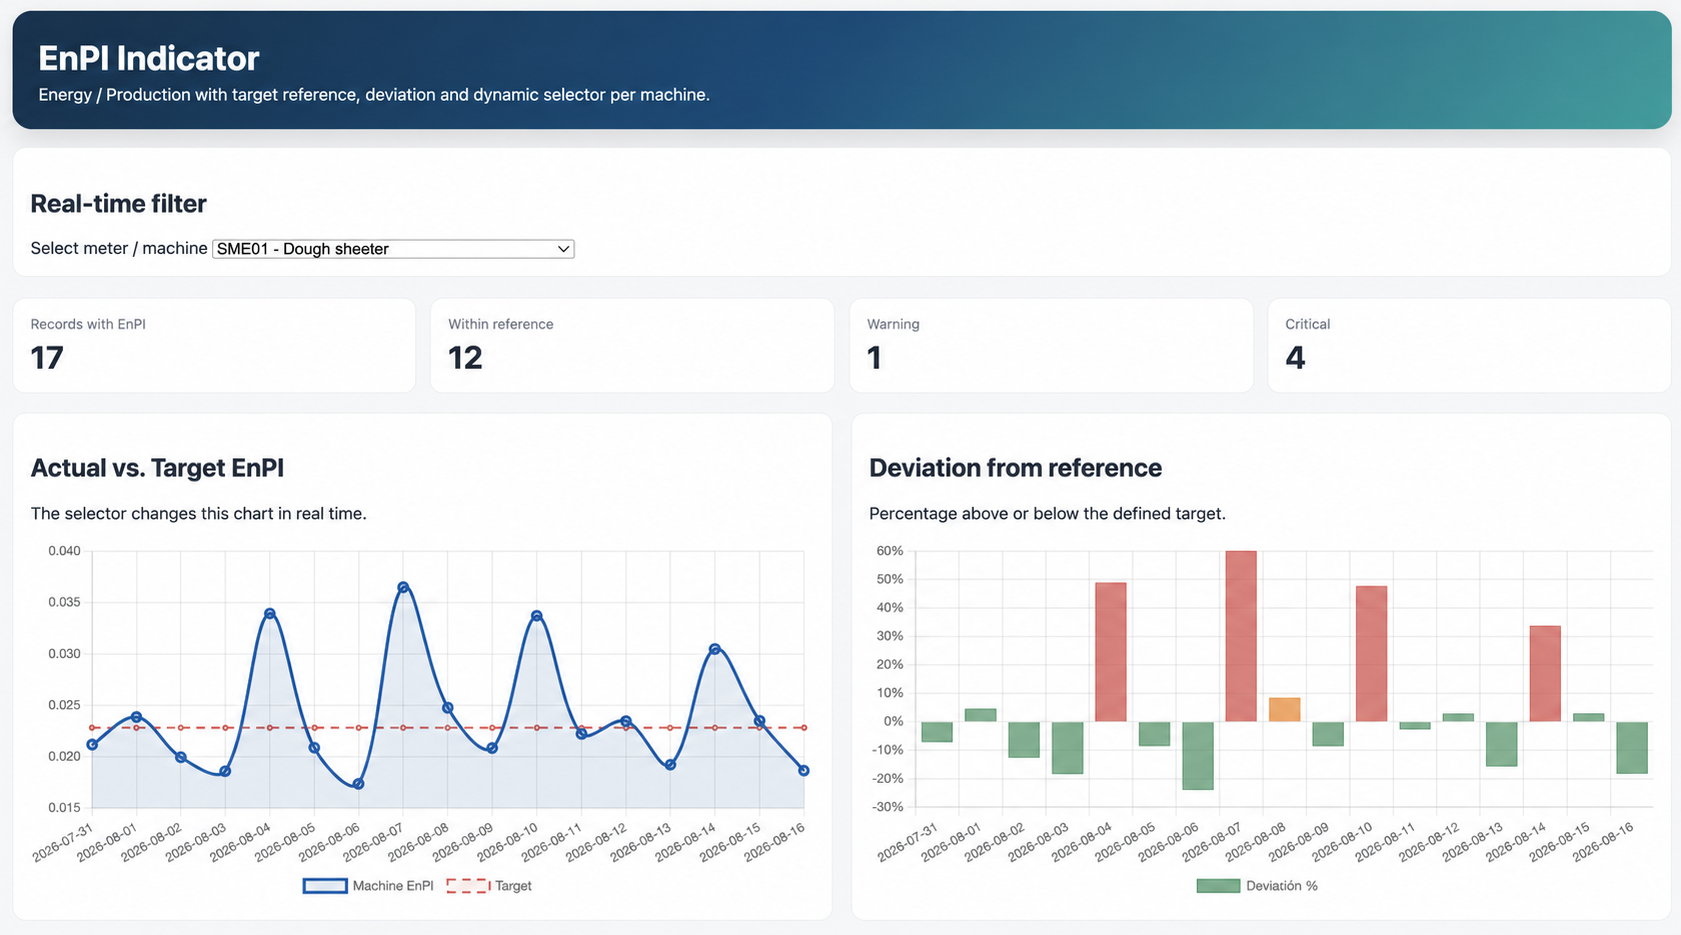
\includegraphics[width=0.7\textwidth]{figures/enpi_dashboard_sme01_dough_sheeter.png}
\caption{EnPI Operational dashboard for the anonymized food-sector SME traceability case. The system compiles 17 daily EnPI records for the monitored dough sheeter: 12 days labeled green, one warning day, and four critical days according to the defined operational rule; these labels are not validated diagnoses. The left panel shows daily EnPI versus the operational target, and the right panel shows the percentage deviation from the reference.}
\label{fig:enpi-dashboard-sme}
\end{figure*}

To avoid repeating a long operational log in the text body, we provide the full 17-day daily log in the public reproducibility repository and summarize the supporting operational material in the Supplementary Material. The aggregate case evidence is 
reported in Table~\ref{tab:caso-real-summary} in the manuscript, and four days leading up to critical alerts are reported in Table~\ref{tab:critical-days}. This maintains focus of the main narrative on the traceability mechanism and the decision-relevant deviations whilst keeping the full log available for audit.

\subsection{Implementation Context for Traceable Sensing}
\label{sec:functional-implementation}

The functional implementation is described only to the extent that it enables traceable sensing. The platform handles organizational units (company/office/facility), metering locations within the organization (metering point/facility), consumption records for each metering point, IoT readings, production/consumption at the point, references to the target, and EnPI factors. Here, manual and i.S. oT. sources are input to the energy database in the process under review; production records provide the operational denominator, and the analytical module computes energy performance against organization-determined references. The production module, which is presented in Supplementary Fig. S2, enables a user to record the quantities produced related to a plant, machine, day or operational unit. This is required because the sensing node alone can only provide electrical readings; EnPI needs a compatible production denominator. 
The operational case dashboard in Figure~\ref{fig:enpi-dashboard-sme} shows this analysis layer with anonymized data, including daily EnPI, reference, and resulting alert status. Supplementary Fig. S4 displays the dashboard for examining consumption records, raw IOT readings, and validation/linking states. 

\section{Discussion}
\label{sec:discussion}
This work should be understood as a contribution of the sensor system rather than a generic software-platform solution. The concurrent measurement campaign provides quantitative proof for the single-phase node under laboratory conditions, and the workflow shows how the resulting readings can maintain provenance through EnPI calculation. Thus, the implementation serves as the data provenance and indicator layer for the represented sensing node. Direct power and interval-energy measurements are more compelling because, to the best of our knowledge, they do not rely on deriving a reference power from other Metrel measurements. However, more work remains to accurately predict long-term stability, energy accuracy at the billing level, and benefits at the plant scale.
This paper differs from those that focus primarily on smart-meter hardware because it investigates integrating a prototyped measurement layer with data provenance and production context. The difference is one of scale of the evidence and not a matter of whether prior platforms can be adapted to similar integrations. An organization, you know, can always start with the records they have and add on IoT metering wherever it makes sense. The claim here is more subdued: in the validated single-phase scenario, the characterized node can enable a traceable energy-performance indicator (EnPI) flow.
This limitation is particularly significant for the majority of the adverse test cases. A commercial sensor–based low-cost node is not a panacea for all operating conditions and certainly is not to be considered as a replacement for a reference-grade power quality analyzer. It is only a somewhat narrowly focused instrument for cheaply measuring the energy consumption of a particular piece of equipment. Before using its readings for energy-intensity metrics, early screening, or further monitor-related decisions, ensure it is suitable for the intended use. 

Tests at no load and very low power help establish those boundaries. They indicate that proportional measurements may be unreliable at low power and that a properly characterized reference analyzer remains necessary in such cases. These tests, however, do not represent the loads that usually drive industrial energy-performance indicators. The controlled heating, tool, and mixed-load tests provide direct comparisons at power levels more relevant to practical applications. In a separate food-sector machine case, stored readings from the node were used to reconstruct an operational EnPI; this case does not demonstrate measurement accuracy against a Metrel analyzer for that industrial machine.
Using an EnPI as the operational output moves the focus from total energy consumption to energy use in relation to production. Such criteria may be used to allow for comparisons between time periods, machines or work centers only if the production units, the windows of observation, the boundaries of measurement and the relevant operating conditions are the same for all those comparisons; those wider comparisons were not validated in this work. In the food-sector case under pseudonymization, adjusted IoT measurements and daily energy were associated with a constant production quantity of 44 kg/day, declared by the enterprise, for 17 days of production. The constant denominator was provided by the enterprise and was not verified as representing daily throughput. 
We compared the values descriptively with literature values for kneading and dough preparation, which are more contextual than universal benchmarks \cite{ref22,ref23}.
This case study demonstrates calculation traceability but does not attempt to explain the underlying reasons for the observed changes. Rule-based alerts can also indicate when energy intensity is much higher than anticipated. The denominator did not change throughout the monitoring period (i.e., 44 kg per day). Hence, fluctuations in the EnPI per day are only caused by variations in (reconstructed) energy data. Although actual production may have varied, this cannot be verified, as there was no independent measurement of throughput. The configured critical threshold was exceeded on four days, with deviations from the selected reference ranging from 33.67\% to 59.99\%. The purpose of these alerts was not to show inefficiency or to determine the root cause of inefficiency. Rather, they provide a time-stamped record that can be used, along with local knowledge, to guide follow-up actions. Potential areas for investigation could be variations in dough batches, idle times, cleaning, schedules, machine loading, or workload. Thus, the EnPI should be considered a support and traceability tool for decision-making, not a standalone diagnostic system. 

These limitations are recognized in the paper and determine the limits of what can be reasonably claimed. Testing at a single measurement point is not representative of an industrial environment, particularly one with high-power motors, three-phase equipment, variable-frequency drives, transient loads, or electrical noise. The food-sector SME example is an EnPI tracking and alert follow-up case study, but it is not a statistical study of multiple companies, nor is it an effort to control for every variable that may influence a specific consumption. The paper said that daily production was constant at 44 kg, but did not independently verify this number. Using a fixed denominator improves traceability, but the case does not demonstrate EnPI behavior as a function of production volume. The study did not independently measure dough type, number of passes, effective load, waiting time, cleaning periods, or intermittent machine usage.
The paper also does not validate simultaneous running of multiple nodes or the long-term field reliability of the new buffering firmware.We may add a high-current single-phase version and a three-phase panel version as scalability extensions, but the focus of the output should be on experimentally validated low-cost sensing and traceable measurement-to-indicator computation. 

\subsection{Answers to the Evaluation Questions}
\label{subsec:rq-answers}
\textbf{RQ1 (measurement agreement).} The valid loaded observations that are synchronized enable quantitative evaluation of agreement for the examined single-phase operating envelope. For the real active power, the combined MAE was 11.408 W, and the average bias was $-11.034$~W across $9,119$ valid loaded pairs. These aggregate results do not imply equal relative accuracy at zero load or very low power, nor do they constitute a formal uncertainty budget or certification. Voltage, current, frequency, and power-factor comparisons must be made within their own valid reference channels and observed scenarios, not as a generalization to an industrial load type. 

\textbf{RQ2 (traceable EnPI calculation).} The separate 17-day food-sector case demonstrates that stored IoT readings can be associated with a machine, observation periods, reconstructed daily energy, and enterprise-declared production to calculate and display a machine-level kWh/kg indicator. This is evidence of a functioning provenance-aware calculation workflow, not an independent validation of the 44~kg/day production values, a Metrel-referenced accuracy trial at the industrial site, or proof of energy savings. Thus, the two evaluation questions are supported by complementary but nonidentical datasets, and no end-to-end industrial metrological validation is claimed.

\section{Limitations}
\label{sec:limitations}
\subsection{Measurement and Reference Scope}
The characterization used a single low-cost single-phase sensing implementation and a limited set of controlled electrical loads. It does not address device-to-device repeatability, long-term drift, performance with three-phase equipment, variable-frequency drives, high-current motors, or industrial electromagnetic disturbances. The Metrel MI2883 served as the operational comparison reference, but the reported errors and bootstrap intervals do not constitute a full measurement-uncertainty budget or a formal calibration of EnPi \cite{r2_gum,r2_vim,r2_bland}.

\subsection{Acquisition Continuity and Energy Resolution}
We conducted a continuity check and found 15 gaps across scenarios, corresponding to 210 missing EnPi readings of one second in scenarios 000, 002, 007, and 009. The intervals were 20, 10, 20, and 160 seconds, respectively. The reference-instrument data were available at these times, but the server export lacked EnPi measurements with matching timestamps. We excluded the missing points from the per-point agreement calculations and made no effort to fill them in. For integrated energy, we considered only cases where both timestamps coincided. Each gap marked the start of a new segment; we accumulated Metrel interval energy over the retained samples, computed EnPi register changes within each continuous segment, and summed these changes.
The archived records show where the gaps were and how long they were, but not whether they were due to sensing, transmission, storage, or timestamp-matching problems. We implemented an additional buffering stage in the firmware after the campaign; thus, it did not affect the reported measurements. Finally, the 1 Wh resolution of the EnPi register constrains the inferences that can be drawn from short low-energy cases. 

\subsection{Operational Case Boundaries}
This model assumes one dough sheeter will be in use for 17 production days. The company reported a denominator of 44 kg/day but did not actually measure it each day. No independent data were available for product type, machine utilization, idle time, or number of processing passes. The 17.987 kWh (the sum of the observed within-day increments minus the 0.108 kWh inter-day increment) and 748 kg are therefore production-normalized indicators, not explanatory variables based on the causes of efficiency change or demonstrated energy savings \cite{r2_iso50015}. 
\section{Future Work}
\label{sec:future-work}
Future work should incorporate independent sensing nodes, repeated load campaigns, long-term energy accumulation, controlled low-load tests with a valid reference channel, motor loads and variable-frequency drives, and three-phase arrangements. A formal uncertainty budget should include the reference instrument, timing, sensor placement, resolution, and environmental conditions. Controlled experiments of communication failures have to make a distinction between local acquisition, transmission success, records recovered, counter resets, and observations lost. Industrial implementation should gather real production quantities and pertinent operational covariates from several machines and sites instead of normalized baselines or causal interventions or validated energy savings prior to test. Data provenance, synchronization, and secure transport are fundamental design requirements and will be incorporated into standards; however, their inclusion does not attest to experimental validation of all related controls in EnPi \cite{r2_ntp,r2_rfc3339,r2_prov,r2_tls}. Edge processing and multi-node IoT architectures provide further avenues for evaluation beyond the features (capabilities) realized in the present experimental implementation \cite{r2_gubbi,r2_shi}. 
\section{Conclusions}
\label{sec:conclusions}
In this paper, we experimentally characterize EnPi, a cost-efficient single-phase IoT electrical sensing node, and present a traceable workflow for reconstructing machine-level energy performance indicators. The controlled campaign consisted of ten cases and 10,596 temporally paired records (9,119 valid loaded observations), allowing the first direct active-power comparison with the Metrel MI2883. The overall MAE was 11.408 W, RMSE was 23.184 W, and the mean bias was $-11.034$ W. Segment-preserving bootstrap suggested that these estimates are conditionally variable, although it didn’t establish metrological certification. The revised analysis emphasizes why the two measurement bodies should be evaluated using the same segment-matching principle. For case 009, the difference is -1.882\%, from 1,042 matched observations over 11 continuous segments. In another 17-day food-sector case,  analysis replicated an energy use of 17.987 kWh, as opposed to the 748 kg production declared by the business. This yields a production weighted EnPI of approximately 0.0240 kWh/kg, with the median daily EnPI at 0.0222 kWh/kg. These numbers represent the same finite case in different manners, and should not be treated as interchangeable. Since the company assumed constant production, neither measure alone verifies energy efficiency.
In summary, results are generally supportive of the application of operational sensing to the extent allowed by the boundaries established by this work, and illustrate the potential to trace and re-derive measurements as indicators under the conditions examined. The contribution is the demonstrated integration of a defined single-phase sensing node and separate indicator traceability (IT), rather than a novel measurement that achieves a higher tier of accuracy than what is widely considered heterogeneous in prior work. The results do not prove billing-grade accuracy, generalize industrial validation, or energy savings through automated causal diagnosis. 

\supplementary{The supplementary material includes the detailed literature synthesis, functional-layer description, platform and traceability views, bill of materials of the implemented EnPi PCB, reproducibility information, firmware buffering logic, direct-power and interval-energy analysis files, additional error visualizations, and supporting records for the 17-day operational case.}
\authorcontributions{Conceptualization, A.V., A. M. and I.D.; methodology, A.V., and A. M.; software, A.V. and A. M.; validation, A.V. and I.D.; formal analysis, A.V. and A. M.; investigation, A.V. and A. M.; data curation, A.V. and A. M.; writing---original draft preparation, A.V. and A. M.; writing---review and editing, A. M., I.D. and J.M.S.; visualization, A.V. and A. M.; supervision, I.D. and J.M.S.; project administration, I.D. All authors have read and agreed to the published version of the manuscript.}
\funding{This work was supported by the Centre for Innovation in Technology and Design of Materials for the Built Environment (CIMAC), ANID CTI250005.}

\institutionalreview{Not applicable.}

\informedconsent{Not applicable. The operational case used anonymized machine-level energy and production records and did not involve human participants or identifiable personal data.}

\dataavailability{The data and materials supporting this study are available in the validated EnPi repository at \url{https://github.com/The-Terial/Enpi}. The repository contains the experimental and operational datasets, synchronized comparison records, analysis scripts, firmware source code, and supporting documentation required to reproduce the reported EnPi--Metrel comparisons, bootstrap sensitivity analysis, communication-gap audit, figures, tables, and 17-day operational calculations. Operational records are anonymized and contain no personally identifiable information.}

\acknowledgments{The authors acknowledge the participating food-sector SME for providing the anonymized operational setting used in the bounded industrial demonstration.}

\conflictsofinterest{The authors declare no conflicts of interest.}
\quad
\section{References}
\begin{thebibliography}{99}
\bibitem{ref1} M. U. Saleem, M. R. Usman, and M. Shakir, "Design, Implementation, and Deployment of an IoT Based Smart Energy Management System," IEEE Access, vol. 9, pp. 59649-59664, 2021, doi: 10.1109/ACCESS.2021.3070960.
\bibitem{ref2} M. Ullah, A. Narayanan, A. Wolff, and P. H. J. Nardelli, "Industrial Energy Management System: Design of a Conceptual Framework Using IoT and Big Data," IEEE Access, vol. 10, pp. 110557--110567, 2022, doi: 10.1109/ACCESS.2022.3215167.
\bibitem{ref3} Y. Li, Z. Sun, L. Han, and N. Mei, "Fuzzy Comprehensive Evaluation Method for Energy Management Systems Based on an Internet of Things," IEEE Access, vol. 5, pp. 21312-21322, 2017, doi: 10.1109/ACCESS.2017.2728081.
\bibitem{ref4} M. U. Saleem, M. R. Usman, M. A. Yaqub, A. Liotta, and A. Asim, "Smarter Grid in the 5G Era: Integrating the Internet of Things With a Cyber-Physical System," IEEE Access, vol. 12, pp. 34002--34018, 2024, doi: 10.1109/ACCESS.2024.3372379.
\bibitem{ref5} S. Kim, S. Lee, M. Kim, and Y. Kwon, "A Web Application Framework for Battery Health Prediction in Industrial IoT Networks," Journal of Web Engineering, vol. 24, no. 6, pp. 943-972, 2025, doi: 10.13052/jwe1540-9589.2464.
\bibitem{ref6} S. M. A. A. Abir, A. Anwar, J. Choi, and A. S. M. Kayes, "IoT-Enabled Smart Energy Grid: Applications and Challenges," IEEE Access, vol. 9, pp. 50961-50981, 2021, doi: 10.1109/ACCESS.2021.3067331.
\bibitem{ref7} Y. Santo, A. Abelem, A. Riker, and E. E. Tsiropoulou, "Integrating Data Privacy and Energy Management in Smart Cities With Partial Sustainable IoT Networks," IEEE Access, vol. 13, pp. 33176--33188, 2025, doi: 10.1109/ACCESS.2025.3541213.
\bibitem{ref8} O. Said, Z. Al-Makhadmeh, and A. Tolba, "EMS: An Energy Management Scheme for Green IoT Environments," IEEE Access, vol. 8, pp. 44983-44998, 2020, doi: 10.1109/ACCESS.2020.2976641.
\bibitem{ref9} B. Safaei, M. Peiravian, and M. Siamaki, "Eco-Friendly IoT: Leveraging Energy Harvesting for a Sustainable Future," IEEE Sensors Reviews, vol. 2, pp. 32--75, 2025, doi: 10.1109/SR.2025.3552043.
\bibitem{ref10} L. N. H. Pham, A. Shrestha, C. Sharma, and F. Gonzalez-Longatt, "Digital Twins and Cyber-Physical Systems Toward the Digitalization of Power and Energy Systems," IEEE Transactions on Technology and Society, vol. 6, no. 4, pp. 393--410, 2025, doi: 10.1109/TTS.2025.3615624.
\bibitem{ref11} M. S. Ahmad, N. N. Mansor, H. Mokhlis, K. Naidu, H. Mohamad, and F. Ramadhani, "Demand Response Program Toward Sustainable Power Supply: Current Status, Challenges, and Prospects in Malaysia," IEEE Access, vol. 13, pp. 34706--34731, 2025, doi: 10.1109/ACCESS.2025.3541841.
\bibitem{ref12} K. Shafique, B. A. Khawaja, F. Sabir, S. Qazi, and M. Mustaqim, "Internet of Things (IoT) for Next-Generation Smart Systems: A Review of Current Challenges, Future Trends and Prospects for Emerging 5G-IoT Scenarios," IEEE Access, vol. 8, pp. 23022-23040, 2020, doi: 10.1109/ACCESS.2020.2970118.
\bibitem{ref13} J. S. Yalli, M. H. Hasan, and A. A. Badawi, "Internet of Things (IoT): Origins, Embedded Technologies, Smart Applications, and Its Growth in the Last Decade," IEEE Access, vol. 12, pp. 91357--91382, 2024, doi: 10.1109/ACCESS.2024.3418995.
\bibitem{ref14} M. Soula, B. Mbarek, and A. Meddeb, "A Real-Time Trust Management Model Using Digital Twin in IoT Networks," IEEE Access, vol. 12, pp. 183326--183343, 2024, doi: 10.1109/ACCESS.2024.3506870.
\bibitem{ref15} A. Bounceur et al., "Phygital Twin IoT: A Hardware-Software Decomposition Architecture for Scalable and Secure Digital Twin IoT Systems," IEEE Open Journal of the Computer Society, vol. 7, pp. 755--768, 2026, doi: 10.1109/OJCS.2026.3681725.
\bibitem{ref16} A. Velez-Estevez, L. Gutierrez-Madronal, and I. Medina-Bulo, "IoT-TEG 4.0: A New Approach 4.0 for Test Event Generation," IEEE Transactions on Reliability, vol. 71, no. 3, pp. 1368--1380, 2022, doi: 10.1109/TR.2021.3087781.
\bibitem{ref17} M. S. Yaraziz and R. Hill, "Federated Q-Learning-Based Optimization for Resource Allocation in Industrial IoT Networks," IEEE Access, vol. 13, pp. 188880--188891, 2025, doi: 10.1109/ACCESS.2025.3624919.
\bibitem{ref18} H. Zhu, K. Ouahada, and A. M. Abu-Mahfouz, "Peer-to-Peer Energy Trading in Smart Energy Communities: A Lyapunov-Based Energy Control and Trading System," IEEE Access, vol. 10, pp. 42916--42932, 2022, doi: 10.1109/ACCESS.2022.3167828.
\bibitem{ref19} International Organization for Standardization, ISO 50001:2018, Energy management systems --- Requirements with guidance for use, Geneva, Switzerland: ISO, 2018.
\bibitem{ref20} International Organization for Standardization, ISO 50006:2023, Energy management systems --- Evaluating energy performance using energy performance indicators and energy baselines, Geneva, Switzerland: ISO, 2023.
\bibitem{ref21} G. W. Hart, ``Nonintrusive Appliance Load Monitoring,'' Proceedings of the IEEE, vol. 80, no. 12, pp. 1870--1891, Dec. 1992, doi: 10.1109/5.192069.
\bibitem{ref22} M. Briceño-León, D. Pazmiño-Quishpe, J.-M. Clairand, and G. Escrivá-Escrivá, ``Energy Efficiency Measures in Bakeries toward Competitiveness and Sustainability--Case Studies in Quito, Ecuador,'' Sustainability, vol. 13, no. 9, Art. no. 5209, 2021, doi: 10.3390/su13095209.
\bibitem{ref23} F. Paschino and F. Gambella, ``Comparison between traditional and industrial plants used for production of `carasau' bread and evaluation of final products,'' Applied Engineering in Agriculture, vol. 23, no. 1, pp. 65--70, 2007, doi: 10.13031/2013.22319.
\bibitem{ref24} J. Varela-Aldás, S. Silva, and G. Palacios-Navarro, ``IoT-Based Alternating Current Electrical Parameters Monitoring System,'' Energies, vol. 15, no. 18, Art. no. 6637, 2022, doi: 10.3390/en15186637.
\bibitem{ref25} International Electrotechnical Commission, IEC 62053-21:2020, Electricity metering equipment --- Particular requirements --- Part 21: Static meters for AC active energy (classes 0,5, 1 and 2), Geneva, Switzerland: IEC, 2020.
\bibitem{ref26} M. Jamshidi, ``System of Systems Engineering---New Challenges for the 21st Century,'' IEEE Aerospace and Electronic Systems Magazine, vol. 23, no. 5, pp. 4--19, May 2008, doi: 10.1109/MAES.2008.4523909.
\bibitem{ref27} D. Minoli, K. Sohraby, and B. Occhiogrosso, ``IoT Considerations, Requirements, and Architectures for Smart Buildings---Energy Optimization and Next-Generation Building Management Systems,'' IEEE Internet of Things Journal, vol. 4, no. 1, pp. 269--283, Feb. 2017, doi: 10.1109/JIOT.2017.2647881.
\bibitem{ref28} G. Bedi, G. K. Venayagamoorthy, R. Singh, R. R. Brooks, and K.-C. Wang, ``Review of Internet of Things (IoT) in Electric Power and Energy Systems,'' IEEE Internet of Things Journal, vol. 5, no. 2, pp. 847--870, Apr. 2018, doi: 10.1109/JIOT.2018.2802704.
\bibitem{r2_gum} Joint Committee for Guides in Metrology, \emph{Evaluation of Measurement Data---Guide to the Expression of Uncertainty in Measurement}, JCGM 100:2008, 2008, doi: 10.59161/JCGM100-2008E.
\bibitem{r2_vim} Joint Committee for Guides in Metrology, \emph{International Vocabulary of Metrology---Basic and General Concepts and Associated Terms}, JCGM 200:2012, 2012, doi: 10.59161/JCGM200-2012.
\bibitem{r2_iso50015} International Organization for Standardization, \emph{ISO 50015:2014---Energy Management Systems---Measurement and Verification of Energy Performance of Organizations---General Principles and Guidance}, 2014.
\bibitem{r2_kunsch} H. R. K\"unsch, ``The jackknife and the bootstrap for general stationary observations,'' \emph{Annals of Statistics}, vol. 17, no. 3, pp. 1217--1241, 1989, doi: 10.1214/aos/1176347265.
\bibitem{r2_politis} D. N. Politis and J. P. Romano, ``The stationary bootstrap,'' \emph{Journal of the American Statistical Association}, vol. 89, no. 428, pp. 1303--1313, 1994, doi: 10.1080/01621459.1994.10476870.
\bibitem{r2_ntp} D. Mills, J. Martin, J. Burbank, and W. Kasch, \emph{Network Time Protocol Version 4: Protocol and Algorithms Specification}, RFC 5905, 2010, doi: 10.17487/RFC5905.
\bibitem{r2_prov} T. Lebo, S. Sahoo, and D. McGuinness, \emph{PROV-O: The PROV Ontology}, W3C Recommendation, 2013.
\bibitem{r2_tls} E. Rescorla, \emph{The Transport Layer Security (TLS) Protocol Version 1.3}, RFC 8446, 2018, doi: 10.17487/RFC8446.
\bibitem{r2_bland} J. M. Bland and D. G. Altman, ``Statistical methods for assessing agreement between two methods of clinical measurement,'' \emph{The Lancet}, vol. 327, no. 8476, pp. 307--310, 1986, doi: 10.1016/S0140-6736(86)90837-8.
\bibitem{r2_hyndman} R. J. Hyndman and A. B. Koehler, ``Another look at measures of forecast accuracy,'' \emph{International Journal of Forecasting}, vol. 22, no. 4, pp. 679--688, 2006, doi: 10.1016/j.ijforecast.2006.03.001.
\bibitem{r2_rfc3339} G. Klyne and C. Newman, \emph{Date and Time on the Internet: Timestamps}, RFC 3339, 2002, doi: 10.17487/RFC3339.
\bibitem{r2_gubbi} J. Gubbi, R. Buyya, S. Marusic, and M. Palaniswami, ``Internet of Things (IoT): A vision, architectural elements, and future directions,'' \emph{Future Generation Computer Systems}, vol. 29, no. 7, pp. 1645--1660, 2013, doi: 10.1016/j.future.2013.01.010.
\bibitem{r2_shi} W. Shi, J. Cao, Q. Zhang, Y. Li, and L. Xu, ``Edge Computing: Vision and Challenges,'' \emph{IEEE Internet of Things Journal}, vol. 3, no. 5, pp. 637--646, 2016, doi: 10.1109/JIOT.2016.2579198.
\bibitem{r2_khasawneh2025} H. J. Khasawneh, R. Al Asbahi, A. W. Alzariqi, D. R. Al Qada, A. Bujuk, M. A. Nawfal, and M. Tareen, ``Industrial IoT-based submetering solution for real-time energy monitoring,'' \emph{Discover Internet of Things}, vol. 5, art. 15, 2025, doi: 10.1007/s43926-025-00110-y.
\bibitem{r2_mirani2024} A. A. Mirani, A. Awasthi, N. O'Mahony, and J. Walsh, ``Industrial IoT-Based Energy Monitoring System: Using Data Processing at Edge,'' \emph{IoT}, vol. 5, no. 4, pp. 608--633, 2024, doi: 10.3390/iot5040027.
\bibitem{r3_sousa2023} E. L. de Sousa, L. A. de Aquino Marques, I. da S. Felix de Lima, A. B. M. Neves, E. N. Cunha, M. E. Kreutz, and A. J. V. Neto, ``Development a Low-Cost Wireless Smart Meter with Power Quality Measurement for Smart Grid Applications'', \emph{Sensors}, vol. 23, no. 16, art. 7210, 2023, doi: 10.3390/s23167210.
\bibitem{r3_openz2018} E. Viciana, A. Alcayde, F. G. Montoya, R. Ba\~nos, F. M. Arrabal-Campos, A. Zapata-Sierra, and F. Manzano-Agugliaro, ``OpenZmeter: An Efficient Low-Cost Energy Smart Meter and Power Quality Analyzer,'' \emph{Sustainability}, vol. 10, no. 11, art. 4038, 2018, doi: 10.3390/su10114038.
\bibitem{r3_khan2024} H. R. Khan, M. Kazmi, Lubaba, M. H. Bin Khalid, U. Alam, K. Arshad, K. Assaleh, and S. A. Qazi, ``A Low-Cost Energy Monitoring System with Universal Compatibility and Real-Time Visualization for Enhanced Accessibility and Power Savings'', \emph{Sustainability}, vol. 16, no. 10, art. 4137, 2024, doi: 10.3390/su16104137.
\bibitem{r3_iotmeter2022} O. Munoz, A. Ruelas, P. Rosales, A. Acu\~na, A. Suastegui, and F. Lara, ``Design and Development of an IoT Smart Meter with Load Control for Home Energy Management Systems,'' \emph{Sensors}, vol. 22, no. 19, art. 7536, 2022, doi: 10.3390/s22197536.
\bibitem{r3_calibration2019} F. Sanchez-Sutil, A. Cano-Ortega, J. C. Hernandez, and C. Rus-Casas, ``Development and Calibration of an Open Source, Low-Cost Power Smart Meter Prototype for PV Household-Prosumers'', \emph{Electronics}, vol. 8, no. 8, art. 878, 2019, doi: 10.3390/electronics8080878.
\bibitem{r3_conti2023} G. Conti, D. Jimenez, A. del Rio, S. Castano-Solis, J. Serrano, and J. Fraile-Ardanuy, ``A Multi-Port Hardware Energy Meter System for Data Centers and Server Farms Monitoring'', \emph{Sensors}, vol. 23, no. 1, art. 119, 2023, doi: 10.3390/s23010119.
\bibitem{r3_iiot2022} R. Bin Mofidul, M. M. Alam, M. H. Rahman, and Y. M. Jang, ``Real-Time Energy Data Acquisition, Anomaly Detection, and Monitoring System: Implementation of a Secured, Robust, and Integrated Global IIoT Infrastructure with Edge and Cloud AI'', \emph{Sensors}, vol. 22, no. 22, art. 8980, 2022, doi: 10.3390/s22228980.
\bibitem{r3_hierarchy2020} B. Beisheim, S. Kr\"amer, and S. Engell, ``Hierarchical aggregation of energy performance indicators in continuous production processes,'' \emph{Applied Energy}, vol. 264, art. 114709, 2020, doi: 10.1016/j.apenergy.2020.114709.
\bibitem{r3_kraft2021} E. Andersson, H. Derneg\aa rd, M. Wall\'en, and P. Thollander, ``Decarbonization of industry: Implementation of energy performance indicators for successful energy management practices in kraft pulp mills'', \emph{Energy Reports}, vol. 7, pp. 1808--1817, 2021, doi: 10.1016/j.egyr.2021.03.009.
\bibitem{r3_piccioni2024} M. Piccioni, F. Martini, C. Martini, and C. Toro, ``Evaluation of Energy Performance Indicators and Energy Saving Opportunities for the Italian Rubber Manufacturing Industry'', \emph{Energies}, vol. 17, no. 7, art. 1584, 2024, doi: 10.3390/en17071584.
\bibitem{r3_korea2021} H.-S. Shim and S.-J. Lee, ``Investigating the Use of Energy Performance Indicators in Korean Industry Sector'', \emph{Journal of the Korea Academia-Industrial Cooperation Society}, vol. 22, no. 3, pp. 707--725, 2021, doi: 10.5762/KAIS.2021.22.3.707.
\bibitem{r3_rubber2020} F. M. Kanchiralla, N. Jalo, S. Johnsson, P. Thollander, and M. Andersson, ``Energy End-Use Categorization and Performance Indicators for Energy Management in the Engineering Industry'', \emph{Energies}, vol. 13, no. 2, art. 369, 2020, doi: 10.3390/en13020369.
\bibitem{r3_atenea2025} A. Ferraro, G. Bruni, M. Salvio, M. Marroccoli, A. Telesca, C. Martini, F. A. Tocchetti, and A. D'Angola, ``ATENEA4SME: Industrial SME Self-Evaluation of Energy Efficiency'', \emph{Energies}, vol. 18, no. 15, art. 4094, 2025, doi: 10.3390/en18154094.
\bibitem{r3_review2024} B. Ioshchikhes, M. Frank, and M. Weigold, ``A Systematic Review of Expert Systems for Improving Energy Efficiency in the Manufacturing Industry'', \emph{Energies}, vol. 17, no. 19, art. 4780, 2024, doi: 10.3390/en17194780.
\bibitem{r3_enpi2026} Y. Castillo Alvarez, R. Jim\'enez Borges, J. P. Monteagudo Yanes, A. Y. Resendiz Jaramillo, L. A. I. Carrera, H. Rodr\'iguez-Res\'endiz, and J. Rodr\'iguez-Res\'endiz, ``A Multistage Sufficiency Test for Selecting Energy Performance Indicators in Industry: Beyond $R^{2}$ Toward the Variable Associated with Significant Energy Use'', \emph{Processes}, vol. 14, no. 16, art. 2676, 2026, doi: 10.3390/pr14162676.
\end{thebibliography}

\end{document}
